\documentclass[a4paper,12pt]{article}

\usepackage[scaled=0.92]{helvet}

\usepackage[colorlinks=true, linkcolor=blue]{hyperref}

\usepackage[english]{babel}
\selectlanguage{english}

\usepackage{microtype}
\usepackage{graphicx}
\usepackage{wrapfig}
\usepackage{enumitem}
\usepackage{amsmath}
\usepackage{index}
\usepackage[utf8]{inputenc}
\usepackage[svgnames]{xcolor}
\usepackage{url}
\usepackage{hyperref}
\usepackage{float}
\usepackage{longtable}
\usepackage[toc]{glossaries}

\begin{document}

\begin{titlepage}

\begin{center}
\vspace*{-1.2in}
\begin{figure}[htb]
\begin{center}

\includegraphics[width=10cm]{Concordia_logo.png}
\end{center}
\end{figure}
\begin{Large}
\vspace*{0.3in}
\textbf{Project Report} \\
\end{Large}
\vspace*{0.1in}
\begin{Large}
For\\
\end{Large}
\vspace*{0.1in}

\begin{Large}
\textbf{Deliverable 1} \\
\end{Large}
\vspace*{0.1in}

\begin{Large}
\textbf{iGo} \\
\end{Large}
\vspace*{0.3in}

\begin{large}
\textbf{Submitted By} \\
\vspace*{0.1in}
\begin{tabular}{c}
  Anant Bir Singh\\
  Prabhjot Singh\\
  Piyush Singla\\
  Parth Sonani\\
  Shivam Dipak Soni\\
\end{tabular}\\
\vspace*{0.4in}
\textbf{Submitted to}\\
\vspace*{0.1in}
Prof. Pankaj Kamthan\\
\vspace*{0.3in}

\begin{Large}
\textbf{SOEN 6461 - Software Design Methodologies} \\
\vspace*{0.2in}
\textbf{Concordia University, Montreal, QC}
\end{Large}

\end{large}
\end{center}
\end{titlepage}


\newcommand{\CC}{C\nolinebreak\hspace{-.05em}\raisebox{.4ex}{\tiny\bf +}\nolinebreak\hspace{-.10em}\raisebox{.4ex}{\tiny\bf +}}
\def\CC{{C\nolinebreak[4]\hspace{-.05em}\raisebox{.4ex}{\tiny\bf ++}}}

\tableofcontents
\newpage
\section{Introduction}
The following document will discuss an online ticket vending machine that can be used in Montreal, Quebec, Canada. We will try to understand the different perspectives of the machine using different models and diagrams, which include use case diagrams.
\subsection{Scope}
iGo is an online platform used to help STM users buy tickets and/or recharge their OPUS cards online and maintain a record of the transactions. The development and maintenance of the STM system and the physical STM ticket vending machines located at STM buildings are separate from iGo.
\subsection{Description}
iGo is an online application that can be used to buy tickets and/or to recharge OPUS cards. The conventional method is to buy the tickets from a TVM. A ticket machine, also known as a ticket vending machine (TVM), is a vending machine that produces paper or electronic tickets, or recharges a stored-value card or smart card or the user's mobile wallet, typically on a smartphone. For instance, ticket machines dispense train tickets at railway stations, transit tickets at metro stations and tram tickets at some tram stops and in some trams.  Token machines may dispense the ticket in the form of a token which has the same function as a paper or electronic ticket. The typical transaction consists of a user using the display interface to select the type and quantity of tickets and then choosing a payment method of either cash, credit/debit card or smartcard.\\ \par
The data from the application will be sent to STM (Société de transport de Montréal) through a secure server. Several organizations are involved in iGo, including the Canadian government, the Public Transport Authority (STM), the payment authority, customers, etc. Users can sign up and log in to track their transactions on this platform. Users can only link one OPUS card to their account to avoid fraud and internal complications. Users can check their transaction history and purchases at any time. \\
iGo will provide the following services to its users:
\begin{enumerate}

\item Customers should be able to create an account on iGo using their email address or phone number. 
\item Customers should be able to login into their accounts and link their OPUS cards to their accounts.
\item Customers should be able to purchase tickets/ recharge their cards and pay through Credit/Debit cards.
\item Customers should be able to view their transaction history.
Customers should be able to schedule payments for their OPUS cards.
\item Customers should be able to remove/ add an OPUS card from their account anytime.
\item Customers should be able to add/ delete/ modify their personal information at any time.
\item Guest users should be able to purchase non-rechargeable tickets.\\
\end{enumerate}


iGo is an efficient solution for the big problem that most Montrealers have to face on the first day of every month, i.e. standing in long queues to recharge their cards and face consequences if they forget to do so. It will save time, money and effort by providing the services in a quick manner.

\newpage
\section {Problem Domain Model}
Problem Domain describes the area undergoing analysis, and includes everything that needs to be understood in order to achieve the goal of the project.  This may includes all inputs and outputs of a process, any related systems, and internal and external project stakeholders.
\subsection{Problem domain model of iGo}
\begin{center}
  \makebox[\textwidth]{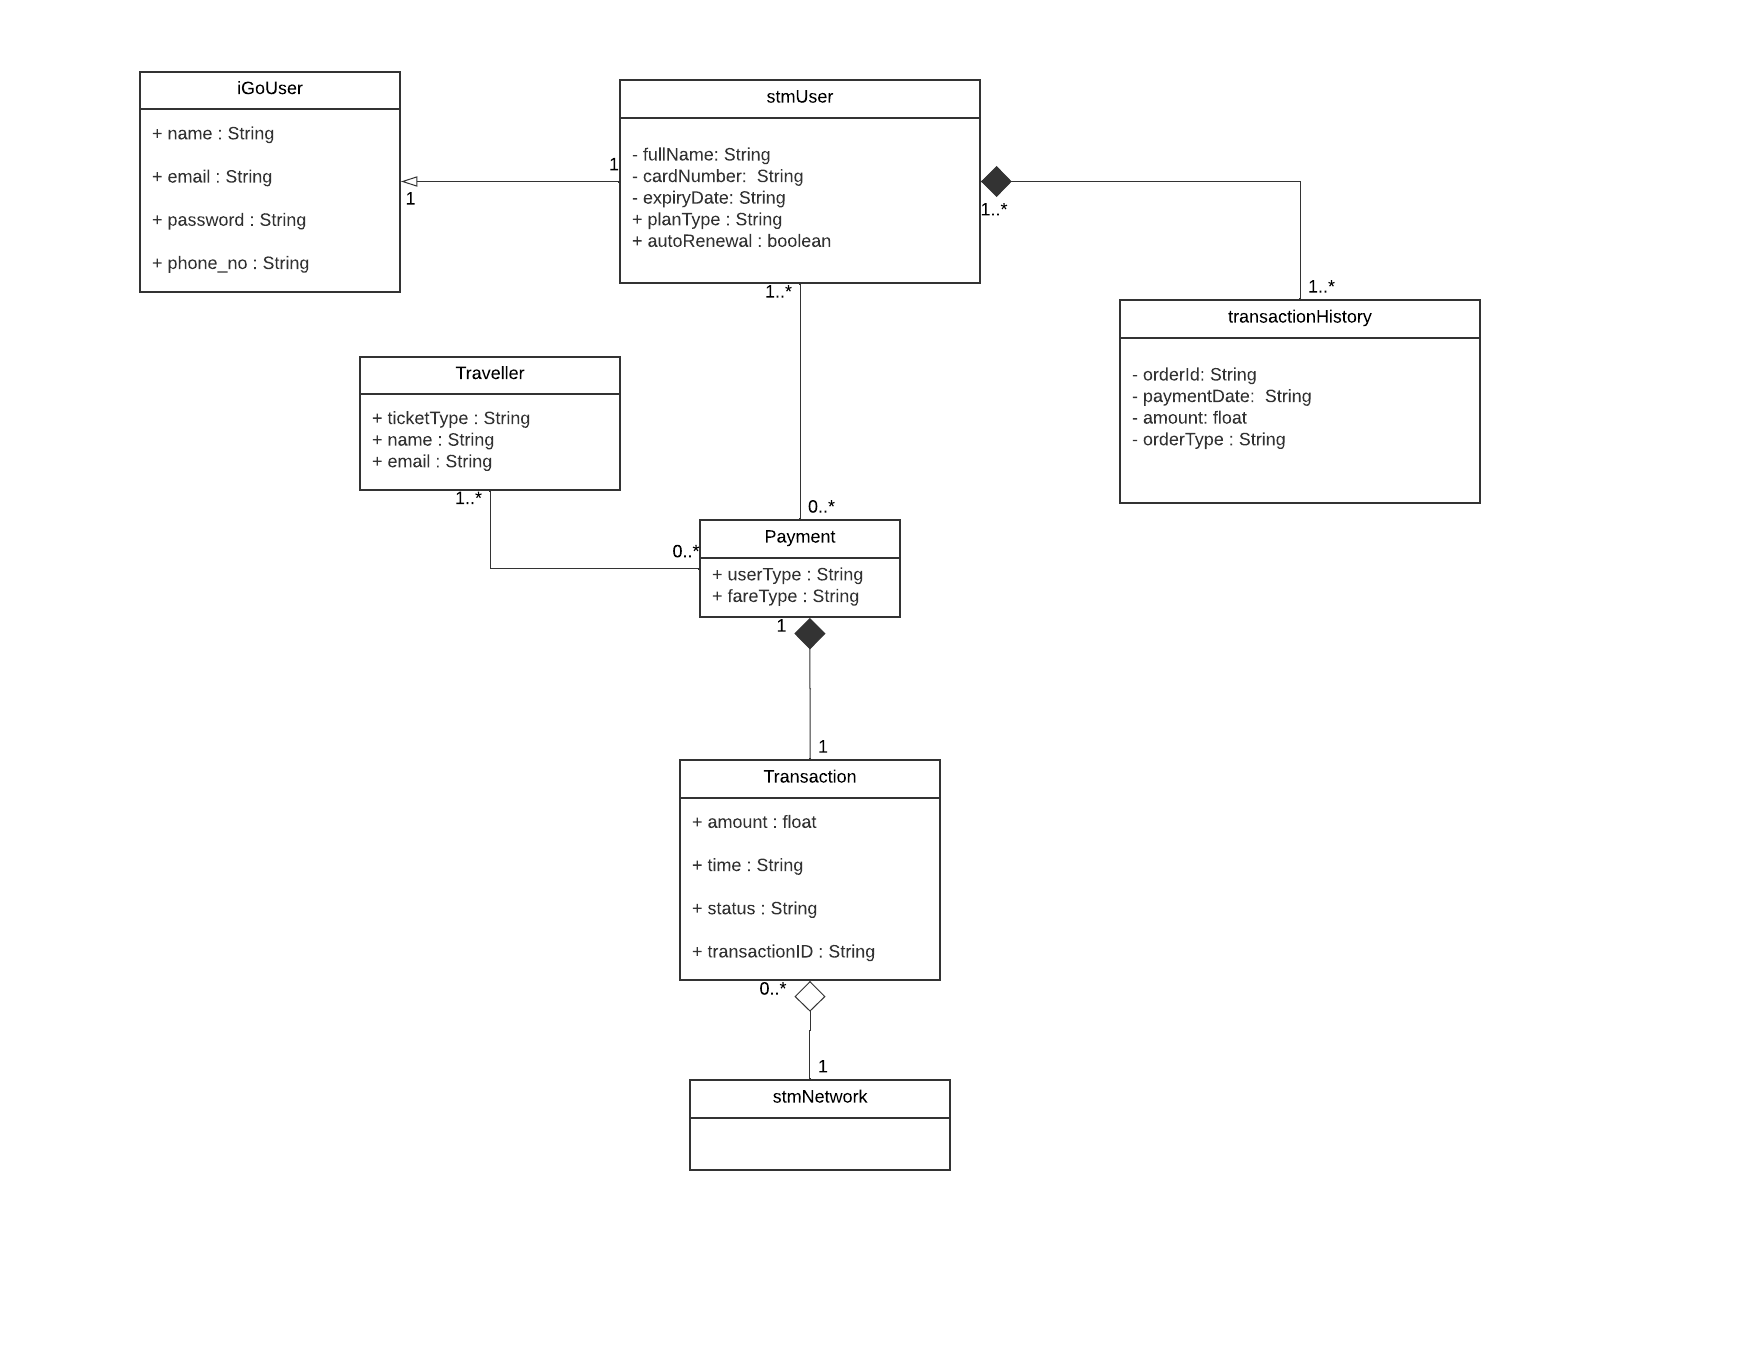
\includegraphics[width=\linewidth]{Problem domain model.png}}
\caption{Problem domain model on iGo system.}
\end{center}
The involved components or classes of the problem domain are as follow
\begin{itemize}[noitemsep]
    \item \textbf{iGo User} It is the potential user of the software developed.
    \item \textbf{stm User} All current STM consumers who utilise the metro service make up this class.
    \item \textbf{Transaction history} This class serves as a representation of all user transactions that have been saved.
    \item \textbf{Traveller} This class of traveller includes everyone who uses the metro but is not a regular citizen or who does not utilise the STM.
    \item \textbf{Payment} This class includes payments made to iGo, which will vary depending on the type of user and the applicable fare.
    \item \textbf{Transaction} The class under the payment class called "transaction" is where the details of the payments would be recorded and where the particular transaction in progress could be seen.
    \item \textbf{STM Network} This is the system that is now in place or the company that manages the stm, to whom data is sent and received.
\end{itemize} \par

Based on the problem domain we can deduct that any travellers or current STM subscribers may sign up for the service, and STM users may open a single account under their names. The iGo will include a capability to remember all of their transactions, and it will also have the ability to be used to buy tickets, allowing users to pay for tickets online directly from the iGo. The current STM network would receive all of the data transmissions.

\newpage
\section {Mindmap}
\subsection{Definition}
A Mind Map is an easy way to brainstorm thoughts organically without worrying about order and structure. It allows you to visually structure your ideas to help with analysis and recall. \\ \par

A Mind Map is a diagram for representing tasks, words, concepts, or items linked to and arranged around a central concept or subject using a non-linear graphical layout that allows the user to build an intuitive framework around a central concept. A Mind Map can turn a long list of monotonous information into a colorful, memorable and highly organized diagram that works in line with your brain's natural way of doing things.\par
\subsection{Use of Mindmap}
For collecting the information required for developing the software we conducted certain interviews of the potential iGo users. The main objective for the interviews were to 
\begin{itemize}[noitemsep]
    \item Identify the users of the metro.
    \item Identify the usage of the metro service.
    \item The problems faced by the users regarding the TVMs
    \item The payment method they use.
    \item Suggestions for changes to the current TVMs they use.
    \item Will they benefit with our product or not?
\end{itemize}
We have created a mind map for deciding the necessary elements or questions on what should be included in the interview. We have used the application Gitmind to generate the mind map for this objective.\\

\begin{center}
  \makebox[\textwidth]{\includegraphics[width=\linewidth]{Mindmap_v3_wo_bg.png}}
\caption{Mind map on deciding the context of questions to be asked to the potential users}
\end{center}

\subsection{Elements in Mind map}
The mind map consists of one central theme which is the interview questions in the current context. The further associations in the following diagrams are the classifications of the categories of questions pertaining to Metro. In this section the categories are listed with one to two questions within them that were asked to the interviewees. 
\subsubsection{Know the users}
\begin{itemize}[noitemsep]
    \item \emph{Tell me your name and age, please.}
\end{itemize}

\subsubsection{Identify type of user}
\begin{itemize}[noitemsep]
    \item \emph{Can you tell me what you do?}
\end{itemize}

\subsubsection{Identify type of transportation used}
\begin{itemize}[noitemsep]
    \item \emph{Do you commute using public transportation or a private vehicle?}
    \item \emph{How frequently do you utilize public transportation?}
\end{itemize}

\subsubsection{Metro usage}
\begin{itemize}[noitemsep]
    \item \emph{Do you know the name of the metro service provider?}
    \item \emph{Do you believe the metro fares are fair to the users?}
\end{itemize}

\subsubsection{Metro ticket}
\begin{itemize}[noitemsep]
    \item \emph{Do you buy tickets or use an OPUS card to ride the metro?}
    \item \emph{How would you proceed if you needed to buy a metro ticket?}
\end{itemize}

\subsubsection{Usage of TVM}
\begin{itemize}[noitemsep]
    \item \emph{Do you think there is enough information present and readable at the TVMs for the metro if you require it?}
    \item \emph{Do you ever have trouble deciding which zone you are in and which zone you want to go to when buying a ticket?}
\end{itemize}

\subsubsection{Payment methods}
\begin{itemize}[noitemsep]
    \item \emph{What form of payment do you find most convenient?}
    \item \emph{Would you prefer an online application to recharge your card or purchase tickets?}
\end{itemize}

\subsubsection{TVM changes/suggestions}
\begin{itemize}[noitemsep]
    \item \emph{Do you think that the OPUS should be recharged online?}
    \item \emph{Are you interested in adding your ticket or OPUS card to your Google or Apple wallet?}
\end{itemize}

\subsection{Interviews}
We have conducted 5 interviews in total. The interviewees are all the existing users of the metro service. We have tried to identify their current ease of access to the TVMs, the problems faced by them due to the TVMs, what changes would they like to see to the current TVM system.

\subsection{Conclusions based on interviews}
The deductions based on the conducted interviews are as follow:
\begin{itemize}
    \item Compared to private transportation, more people use public transportation.
    \item Metro transportation is preferred above bus service by those who use public transportation.
    \item Most people who use the metro commute via it at least two or three times a week and utilize it to get to work or go shopping.
    \item People favour the metro because it runs more frequently and more quickly than other modes of transportation.
    \item Many consider the metro to be a trustworthy and reliable system.
    \item Many are happy with the present fare structure and think it is quite reasonable.
    Although everyone has used a ticket vending machine to buy tickets, they all prefer using their OPUS cards instead.
    \item Aside from the first time, people believe that TVM contain sufficient information and are simple to use.
    \item Consumers find it convenient since there is always an STM booth representative there to assist them with any inquiries they may have about the TVM.
    \item The quantity of TVMs available at a metro station and whether or not the TVMs should be placed outside of the metro station have drawn conflicting opinions.
    \item Many find the ticket zoning system difficult; they must use Google Maps to determine which zone they are in and where they need to travel.
    \item Credit/debit cards are the most practical form of payment for most consumers, while they would prefer to see online payment options in TVMs.
    \item The TVM's authentication and payment security are determined to be extremely reliable and safe.
    \item Given how evolved the technology is, people would like to see the touchscreen interface in TVMs.
    \item Consumers strongly desire that the ticketing process and OPUS card recharging be done online so they don't have to wait in a TVM line.
    \item Consumers appreciated the idea of a monthly subscription model since it would save them time from having to recharge their OPUS cards at the beginning or end of each month.
    \item Many are eager to acquire additional indulgent monthly or yearly passes if they become available.
    \item Consumers prefer "tap to pay" capability in TVM to swiping and entering card information for payment.
    \item Many felt the need for an online solution to buy tickets and recharge their OPUS cards after missing their metro due to an excessive amount of traffic at TVMs at the beginning and end of the month.
    \item People further suggested the improvements they would like to see such as
    \begin{itemize}
        \item the TVMs' UI should be improved and made more user-friendly.
        \item They should introduce online ticket sales since doing so will help them keep up with metro updates too.
        \item After recharging, the change system should either be electronic or use notes rather than money because carrying cash is cumbersome.
    \end{itemize}
\end{itemize}

(Refer to appendix for the transcripts of the interviews)

\newpage
\section{Use Case Model}
A use-case model is a model of how different types of users interact with the system to solve a problem.  As such, it describes the goals of the users, the interactions between the users and the system, and the required behavior of the system in satisfying these goals.
\subsection{Use case model of iGo}
\begin{center}
  \makebox[\textwidth]{\includegraphics[width=\linewidth]{UseCase.png}}
\caption{Use case model of iGo solution.}
\end{center} \par
The use case model for iGo is represented with the help of the use case diagram shown in the figure. It provides an overview of the system's functionalities and requirements from a user's perspective. The use cases and actors for the system are defined below:
 
\begin{itemize}
    \item Actors
    \begin{itemize}
        \item Commuter: This actor represents commuters using the public transit system in Montreal and managing their OPUS cards.
        \item STM system: This actor maintains the user database and provides user and OPUS card-related details to iGo.
        \item Bank: This actor represents the external bank that is used for processing commuter payments
    \end{itemize}
    \item Use Cases
    \begin{itemize}
        \item Register: This use case represents the process of a commuter registering with iGo.
        \item Get Authentication: This use case represents the process of a commuter providing their authentication credentials (username and password) to iGo to access their account and perform various operations.
        \item Authenticate credentials: This use case represents the process of iGo verifying a commuter's authentication credentials from the user database.
        \item Buy new OPUS card: This use case represents the process of a commuter purchasing a new OPUS card from iGo. It includes the 'Select transit type' use case.
        \item Buy non-rechargeable card: This use case represents the process of a commuter purchasing a non-rechargeable ticket from iGo.It includes the 'Select transit type' use case.
        \item Recharge OPUS card: This use case represents the process of a commuter adding funds to an existing rechargeable OPUS card. It includes the 'Select transit type' use case.
        \item Select transit type: This use case represents the process of a user selecting between various transit types (one-way trip, weekly pass, monthly pass, etc.)
        \item Check OPUS validity: This use case represents the process of checking the validity and balance of an OPUS card.
        \item Make payment: This use case represents the process of a commuter making a payment to iGo for their transaction.
    \end{itemize}
\end{itemize}

 This generalizes three use cases: ' Pay with cash,' 'Pay with debit card,' and 'Pay with credit card.'

\newpage
\section{Activity diagrams}
Activity Diagrams describe how activities are coordinated to provide a service which can be at different levels of abstraction. Typically, an event needs to be achieved by some operations, particularly where the operation is intended to achieve a number of different things that require coordination, or how the events in a single use case relate to one another, in particular, use cases where activities may overlap and require coordination. It is also suitable for modeling how a collection of use cases coordinate to represent business workflows.
\subsection{Activity diagrams in iGo}
\begin{enumerate}
\item Activity diagram showing the 
\begin{itemize}
    \item Login
    \item Authentication
\end{itemize}
\begin{center}
  \makebox[\textwidth]{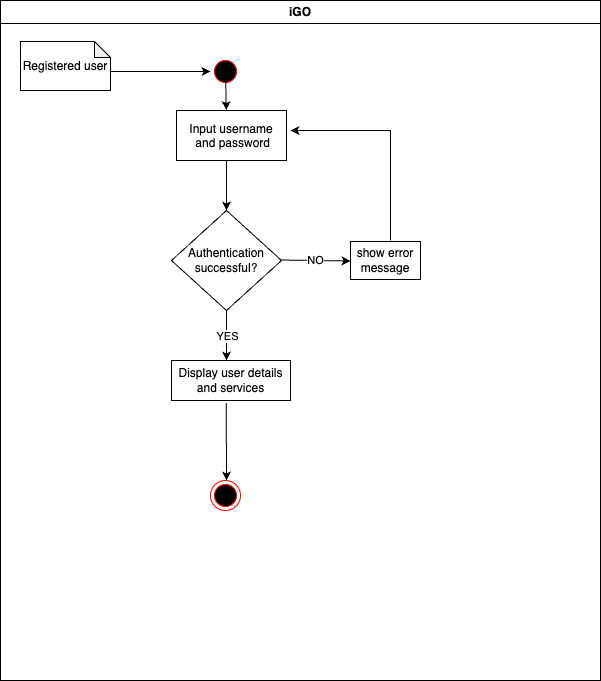
\includegraphics[width=\linewidth]{activity diagram_1.png}}
\end{center}

\item Activities showed in this diagram are\
\begin{itemize}
    \item Buy new OPUS card.
    \item Buy ticket.
    \item Recharge OPUS.
\end{itemize}
\begin{center}
  \makebox[\textwidth]{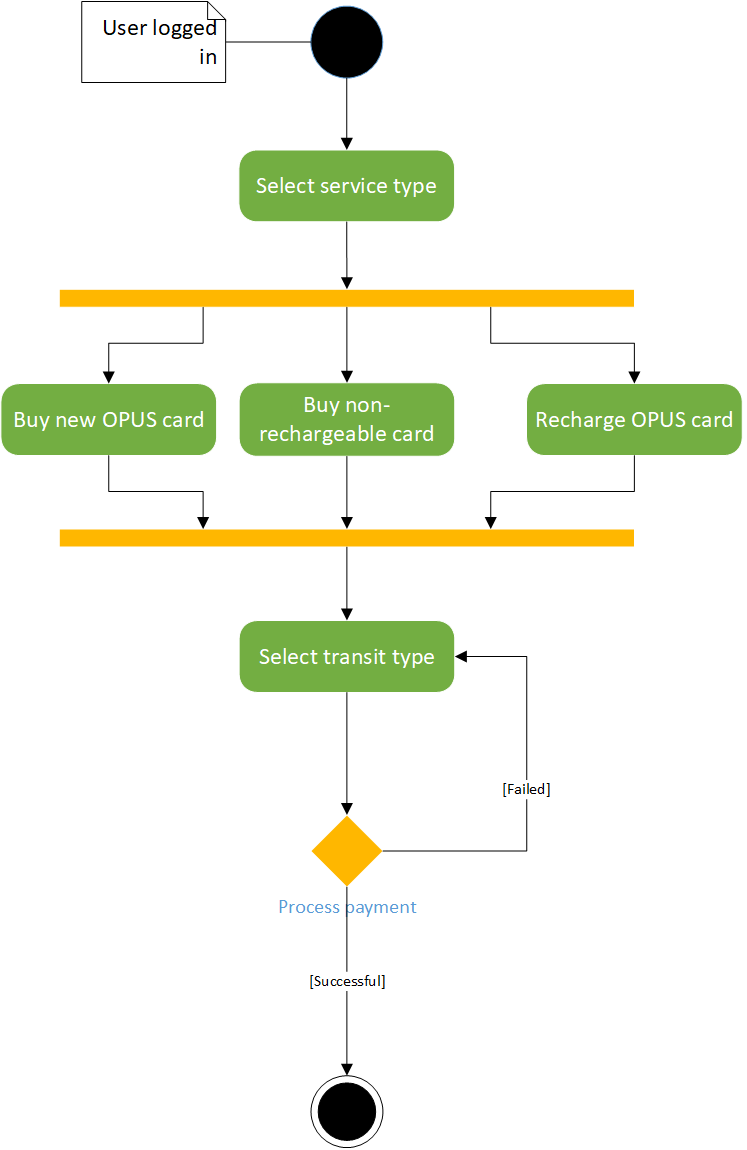
\includegraphics[width=\linewidth]{activity diagram_2.png}}
\end{center}

\item This activity diagram depicts how the authentication is happening for the OPUS card.
\begin{center}
  \makebox[\textwidth]{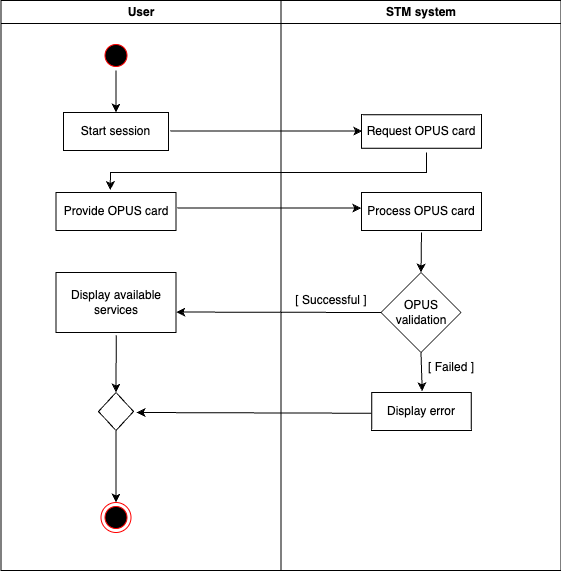
\includegraphics[width=\linewidth]{activity diagram_3.png}}
\end{center}

\item This activity diagram demonstrates the the process of payment through different methods that are suitable for the user.
\begin{center}
  \makebox[\textwidth]{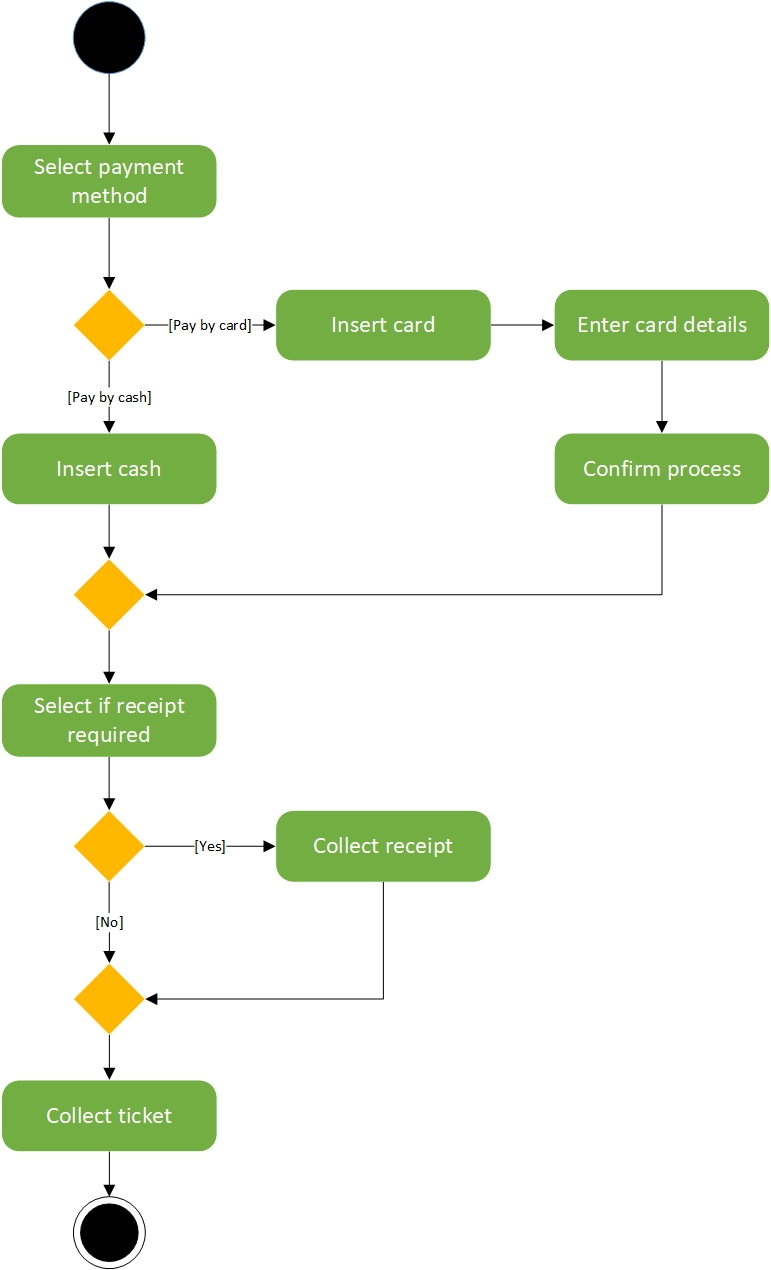
\includegraphics[width=\linewidth]{activity diagram_4.jpeg}}
\end{center}

\item This activity diagram demonstrates the the process of OPUS card validation.
\begin{center}
  \makebox[\textwidth]{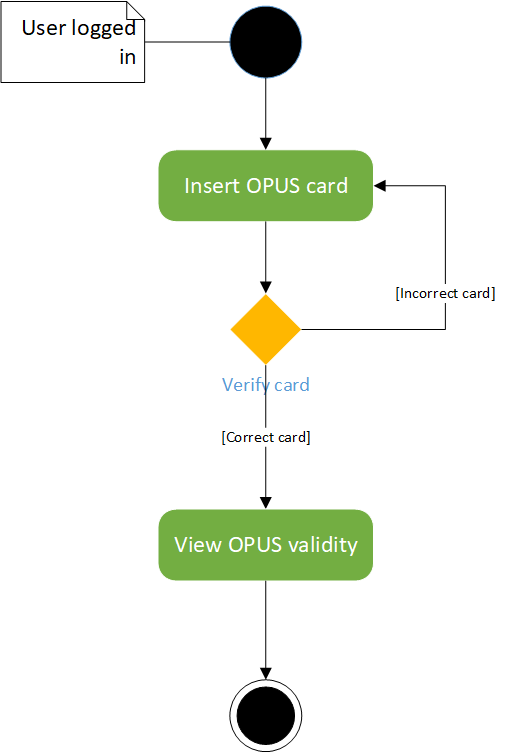
\includegraphics[width=\linewidth]{activity diagram_5.png}}
\end{center}
\end{enumerate}

\newpage
\section{References}
\begin{enumerate}
    \item What is a Ticket Machine [\href{https://en.wikipedia.org/wiki/Ticket_machine}{Ticket Machine}]
    \item What is a  \href{https://www.businessprocessglossary.com/9158/problem-domain#:~:text=1%20Definition,internal%20and%20external%20project%20stakeholders.}{Problem domain model}
    \item What is a \href{https://www.mindmapping.com/mind-map}{Mind map}
    \item What is \href{https://gitmind.com/}{Gitmind} and how to use.
    \item Basics of  \href{https://simplemind.eu/how-to-mind-map/basics/}{Mind mapping}
    \item What is a  \href{https://www.utm.mx/~caff/doc/OpenUPWeb/openup/guidances/concepts/use_case_model_CD178AF9.html#:~:text=A%20use%2Dcase%20model%20is,system%20in%20satisfying%20these%20goals.}{Use case model}
    \item What is an \href{https://www.visual-paradigm.com/guide/uml-unified-modeling-language/what-is-activity-diagram/}{Activity diagram}
\end{enumerate}

\newpage
\section{Appendix}
\subsection{Interview transcripts}
\subsubsection{Interview with Deep Raval}

\hypertarget{interviewer}{%
\subparagraph{{[}00:00:04.890{]} - Interviewer}\label{interviewer}}

Please tell me your name and age?

\hypertarget{interviewee}{%
\subparagraph{{[}00:00:07.570{]} - Interviewee}\label{interviewee}}

Hi, I am Deep Rawal and my age is 22.

\hypertarget{interviewer-1}{%
\subparagraph{{[}00:00:11.010{]} - Interviewer}\label{interviewer-1}}

Can you tell me what do you do?

\hypertarget{interviewee-1}{%
\subparagraph{{[}00:00:12.960{]} - Interviewee}\label{interviewee-1}}

I'm currently a student at Concordia University pursuing masters in
Applied Computer science.

\hypertarget{interviewer-2}{%
\subparagraph{{[}00:00:18.370{]} - Interviewer}\label{interviewer-2}}

Do you commute using public transportation or a private vehicle?

\hypertarget{interviewee-2}{%
\subparagraph{{[}00:00:21.880{]} - Interviewee}\label{interviewee-2}}

Well, I don't have a private vehicle, so whenever I want to go somewhere
far, I use public transport.

\hypertarget{interviewer-3}{%
\subparagraph{{[}00:00:30.810{]} - Interviewer}\label{interviewer-3}}

How frequently do you utilize public transportation?

\hypertarget{interviewee-3}{%
\subparagraph{{[}00:00:34.010{]} - Interviewee}\label{interviewee-3}}

Recently I have not been utilizing it that much, but yeah, I utilize it
maybe once or twice a week.

\hypertarget{interviewer-4}{%
\subparagraph{{[}00:00:42.910{]} - Interviewer}\label{interviewer-4}}

What kind of public transportation do you personally prefer?

\hypertarget{interviewee-4}{%
\subparagraph{{[}00:00:47.710{]} - Interviewee}\label{interviewee-4}}

I prefer Metro because it's fast, convenient, but I might have to take a
bus also. I am open for both of them.

\hypertarget{interviewer-5}{%
\subparagraph{{[}00:00:57.490{]} - Interviewer}\label{interviewer-5}}

Do you know the name of the Metro service provider?

\hypertarget{interviewee-5}{%
\subparagraph{{[}00:01:01.410{]} - Interviewee}\label{interviewee-5}}

I think it's called STM if I'm not wrong.

\hypertarget{interviewer-6}{%
\subparagraph{{[}00:01:03.580{]} - Interviewer}\label{interviewer-6}}

How reliable do you think the Metro is?

\hypertarget{interviewee-6}{%
\subparagraph{{[}00:01:08.950{]} - Interviewee}\label{interviewee-6}}

I would say it is reliable. I have not faced any difficulties in terms
of reliability.

\hypertarget{interviewer-7}{%
\subparagraph{{[}00:01:17.050{]} - Interviewer}\label{interviewer-7}}

Do you believe the Metro fares are fair to the users?

\hypertarget{interviewee-7}{%
\subparagraph{{[}00:01:20.890{]} - Interviewee}\label{interviewee-7}}

Yeah, it is actually fair because for the students they actually give
subsidies, so you have to pay only \$56. So I think that's pretty great.

\hypertarget{interviewer-8}{%
\subparagraph{{[}00:01:31.230{]} - Interviewer}\label{interviewer-8}}

How would you proceed if you needed to buy a Metro ticket?

\hypertarget{interviewee-8}{%
\subparagraph{{[}00:01:35.630{]} - Interviewee}\label{interviewee-8}}

If I wanted to buy a Metro ticket, like separately a ticket, then I
would simply go to a ticket vending machine.

\hypertarget{interviewer-9}{%
\subparagraph{{[}00:01:43.330{]} - Interviewer}\label{interviewer-9}}

Do you buy tickets from the ticket machines?

\hypertarget{interviewee-9}{%
\subparagraph{{[}00:01:47.490{]} - Interviewee}\label{interviewee-9}}

Yeah, but I don't need to buy it now because I have OPUS card.

\hypertarget{interviewer-10}{%
\subparagraph{{[}00:01:52.850{]} - Interviewer}\label{interviewer-10}}

Do you think there is enough information present and readable at the
Tvms for the Metro if you require it?

\hypertarget{interviewee-10}{%
\subparagraph{{[}00:02:01.910{]} - Interviewee}\label{interviewee-10}}

I would say the information is correct, but sometimes it can be a little
ambiguous. But overall it's good.

\hypertarget{interviewer-11}{%
\subparagraph{{[}00:02:11.530{]} - Interviewer}\label{interviewer-11}}

Who do you contact if you have any questions about the Tvm?

\hypertarget{interviewee-11}{%
\subparagraph{{[}00:02:16.810{]} - Interviewee}\label{interviewee-11}}

I would just go to the person in the booth beside the Metro stations and
that but if he's not he or she is not there, I will simply call the STM
helpline.

\hypertarget{interviewer-12}{%
\subparagraph{{[}00:02:28.270{]} - Interviewer}\label{interviewer-12}}

Do you believe that the TVM's current locations are appropriate or
should it also be located somewhere outside of the Metro station?

\hypertarget{interviewee-12}{%
\subparagraph{{[}00:02:36.630{]} - Interviewee}\label{interviewee-12}}

Current locations are okay, but during peak hours or peak days there is
a lot of rush to renew OPUS and get tickets. So it would be great if we
can have ticket vending machine outside of the Metro station, so you can
just go there and get tickets.

\hypertarget{interviewer-13}{%
\subparagraph{{[}00:02:55.600{]} - Interviewer}\label{interviewer-13}}

Did you encounter any problems while using Tvm for the first time?

\hypertarget{interviewee-13}{%
\subparagraph{{[}00:02:59.930{]} - Interviewee}\label{interviewee-13}}

Well, for the first time I encountered a bit of problem. I was confused
which zone should I choose? I had problems with the French language, but
yeah, I figured it out.

\hypertarget{interviewer-14}{%
\subparagraph{{[}00:03:15.390{]} - Interviewer}\label{interviewer-14}}

Do you ever have trouble deciding which zone you are in and which zone
you want to go when buying a ticket?

\hypertarget{interviewee-14}{%
\subparagraph{{[}00:03:23.090{]} - Interviewee}\label{interviewee-14}}

So for the first time, when I was actually renewing my, sorry recharging
for the first time, so I was confused that in which zone I'm in. So
there are a couple of zones and there are many there were many options,
but I figured that the Zone A should be my zone because it was for \$56.
So yeah.

\hypertarget{interviewer-15}{%
\subparagraph{{[}00:03:47.770{]} - Interviewer}\label{interviewer-15}}

What form of payment do you find most convenient?

\hypertarget{interviewee-15}{%
\subparagraph{{[}00:03:51.610{]} - Interviewee}\label{interviewee-15}}

I find NFC payments more convenient because you can just add your card
and you don't have to carry your card and then you can simply do it by
tap and pay.

\hypertarget{interviewer-16}{%
\subparagraph{{[}00:04:02.880{]} - Interviewer}\label{interviewer-16}}

What would you say about TVM's authentication system?

\hypertarget{interviewee-16}{%
\subparagraph{{[}00:04:07.550{]} - Interviewee}\label{interviewee-16}}

I have not faced any issues with that, so I guess it is pretty good.

\hypertarget{interviewer-17}{%
\subparagraph{{[}00:04:12.130{]} - Interviewer}\label{interviewer-17}}

How would you rate payment security with TVMs?

\hypertarget{interviewee-17}{%
\subparagraph{{[}00:04:15.430{]} - Interviewee}\label{interviewee-17}}

Again, I have not faced any issues or security issues for payments, so I
would say it's good.

\hypertarget{interviewer-18}{%
\subparagraph{{[}00:04:23.330{]} - Interviewer}\label{interviewer-18}}

Would you prefer an online application to recharge your card or purchase
tickets?

\hypertarget{interviewee-18}{%
\subparagraph{{[}00:04:28.080{]} - Interviewee}\label{interviewee-18}}

Definitely I would prefer that because then I don't have to go in Tvm
and stand up in line, that would actually waste my time, and if I get
something online, I can do it at my time reliably.

\hypertarget{interviewer-19}{%
\subparagraph{{[}00:04:42.730{]} - Interviewer}\label{interviewer-19}}

What interface do you prefer in Tvm touchscreen or dialpad?

\hypertarget{interviewee-19}{%
\subparagraph{{[}00:04:47.280{]} - Interviewee}\label{interviewee-19}}

Definitely touch screen because it's more intuitive.

\hypertarget{interviewer-20}{%
\subparagraph{{[}00:04:50.270{]} - Interviewer}\label{interviewer-20}}

Would you like to get a monthly subscription paradigm for your recharge?

\hypertarget{interviewee-20}{%
\subparagraph{{[}00:04:55.710{]} - Interviewee}\label{interviewee-20}}

Yeah, I think it would be great. If I can have that. I can just put in
my details and I don't have to worry about it.

\hypertarget{interviewer-21}{%
\subparagraph{{[}00:05:03.410{]} - Interviewer}\label{interviewer-21}}

How would you feel if Tvm offered monthly or annual passes that allowed
you to save time and money?

\hypertarget{interviewee-21}{%
\subparagraph{{[}00:05:09.730{]} - Interviewee}\label{interviewee-21}}

I would definitely consider opting into such offers if I can save money.

\hypertarget{interviewer-22}{%
\subparagraph{{[}00:05:15.690{]} - Interviewer}\label{interviewer-22}}

Are you interested in adding your ticket or Opus card to your Google or
Apple wallet?

\hypertarget{interviewee-22}{%
\subparagraph{{[}00:05:21.130{]} - Interviewee}\label{interviewee-22}}

Yeah, I've been missing this feature, so I wish Opus had such features
so I don't have to carry Opus card.

\hypertarget{interviewer-23}{%
\subparagraph{{[}00:05:28.570{]} - Interviewer}\label{interviewer-23}}

Would you like to see Tvm implement the tap to pay feature?

\hypertarget{interviewee-23}{%
\subparagraph{{[}00:05:32.160{]} - Interviewee}\label{interviewee-23}}

Yeah, definitely. Because currently I don't carry cards with me because
I have them in my mobile wallet. So if Tvm had such system, it would be
great. So I don't have to carry a card with me.

\hypertarget{interviewer-24}{%
\subparagraph{{[}00:05:48.110{]} - Interviewer}\label{interviewer-24}}

How frequently is your lack of access to Tvm preventing you from getting
where you need to be?

\hypertarget{interviewee-24}{%
\subparagraph{{[}00:05:54.850{]} - Interviewee}\label{interviewee-24}}

Not that much.

\hypertarget{interviewer-25}{%
\subparagraph{{[}00:05:57.810{]} - Interviewer}\label{interviewer-25}}

Do you find TVMs busy during office hours or have you ever missed the
Metro because of TVM's excessive rush?

\hypertarget{interviewee-25}{%
\subparagraph{{[}00:06:05.450{]} - Interviewee}\label{interviewee-25}}

Yeah, just recently when I was renewing my OPUS card, there was a lot of
rush and I actually missed one Metro.

\hypertarget{interviewer-26}{%
\subparagraph{{[}00:06:12.290{]} - Interviewer}\label{interviewer-26}}

Do you have any further suggestions for improving the current Tvm
system?

\hypertarget{interviewee-26}{%
\subparagraph{{[}00:06:17.210{]} - Interviewee}\label{interviewee-26}}

Yeah, maybe make UI better and make it even more intuitive, I guess.

\hypertarget{interviewer-27}{%
\subparagraph{{[}00:06:24.090{]} - Interviewer}\label{interviewer-27}}

Thank you.
\newpage
\subsubsection{Interview with Preet Angad}
\hypertarget{interviewer-2}{%
\subparagraph{{[}00:00:00.650{]} - Interviewer 2}\label{interviewer-2}}

Hello.

\hypertarget{interviewee}{%
\subparagraph{{[}00:00:01.570{]} - Interviewee}\label{interviewee}}

Hi.

\hypertarget{interviewer-2-1}{%
\subparagraph{{[}00:00:02.550{]} - Interviewer
2}\label{interviewer-2-1}}

Tell me your name and age, please.

\hypertarget{interviewee-1}{%
\subparagraph{{[}00:00:04.960{]} - Interviewee}\label{interviewee-1}}

I am Preet Angad and my age is 22.

\hypertarget{interviewer-1}{%
\subparagraph{{[}00:00:08.280{]} - Interviewer 1}\label{interviewer-1}}

Can you please tell me what do you do?

\hypertarget{interviewee-2}{%
\subparagraph{{[}00:00:10.550{]} - Interviewee}\label{interviewee-2}}

I'm a graduate student at Concordia.

\hypertarget{interviewer-2-2}{%
\subparagraph{{[}00:00:13.250{]} - Interviewer
2}\label{interviewer-2-2}}

Do you commute using public transportation or a private vehicle?

\hypertarget{interviewee-3}{%
\subparagraph{{[}00:00:17.470{]} - Interviewee}\label{interviewee-3}}

I commute using a public transportation.

\hypertarget{interviewer-1-1}{%
\subparagraph{{[}00:00:19.870{]} - Interviewer
1}\label{interviewer-1-1}}

How frequently do you utilize public transportation?

\hypertarget{interviewee-4}{%
\subparagraph{{[}00:00:22.950{]} - Interviewee}\label{interviewee-4}}

I utilize it every day, almost, yes.

\hypertarget{interviewer-2-3}{%
\subparagraph{{[}00:00:26.220{]} - Interviewer
2}\label{interviewer-2-3}}

Okay, so what kind of public transportation do you personally prefer?

\hypertarget{interviewee-5}{%
\subparagraph{{[}00:00:31.330{]} - Interviewee}\label{interviewee-5}}

I prefer Metro and buses because they are easy to commute.

\hypertarget{interviewer-1-2}{%
\subparagraph{{[}00:00:36.090{]} - Interviewer
1}\label{interviewer-1-2}}

Do you know the name of the Metro service provider?

\hypertarget{interviewee-6}{%
\subparagraph{{[}00:00:38.720{]} - Interviewee}\label{interviewee-6}}

Yes, it's STM, but I don't know the full form of it.

\hypertarget{interviewer-2-4}{%
\subparagraph{{[}00:00:41.860{]} - Interviewer
2}\label{interviewer-2-4}}

Yeah, it's STM. How reliable do you think the Metro is?

\hypertarget{interviewee-7}{%
\subparagraph{{[}00:00:46.270{]} - Interviewee}\label{interviewee-7}}

It's very reliable and very frequent. Yes.

\hypertarget{interviewer-1-3}{%
\subparagraph{{[}00:00:49.680{]} - Interviewer
1}\label{interviewer-1-3}}

Do you believe the Metro fares are fair to the users?

\hypertarget{interviewee-8}{%
\subparagraph{{[}00:00:53.330{]} - Interviewee}\label{interviewee-8}}

Yes, they are quite fair as I also get a student discount, so I get 50\%
off on the fare. Yeah.

\hypertarget{interviewer-2-5}{%
\subparagraph{{[}00:01:01.890{]} - Interviewer
2}\label{interviewer-2-5}}

How would you proceed if you need to buy a Metro ticket?

\hypertarget{interviewee-9}{%
\subparagraph{{[}00:01:07.510{]} - Interviewee}\label{interviewee-9}}

I usually go to the Tvm, which is located at the Metro station. It is
present on each Metro station. And before you enter the Metro, do.

\hypertarget{interviewer-1-4}{%
\subparagraph{{[}00:01:16.730{]} - Interviewer
1}\label{interviewer-1-4}}

You buy tickets or you have an OPUS card to ride the Metro?

\hypertarget{interviewee-10}{%
\subparagraph{{[}00:01:19.770{]} - Interviewee}\label{interviewee-10}}

Yes, I bought an OPUS card. I have an Opus Card registered on my name
and I recharge it every month.

\hypertarget{interviewer-1-5}{%
\subparagraph{{[}00:01:26.570{]} - Interviewer
1}\label{interviewer-1-5}}

Okay.

\hypertarget{interviewer-2-6}{%
\subparagraph{{[}00:01:27.230{]} - Interviewer
2}\label{interviewer-2-6}}

Do you think there is enough information present and readable at the
TVMs for the Metro if you require it?

\hypertarget{interviewee-11}{%
\subparagraph{{[}00:01:34.430{]} - Interviewee}\label{interviewee-11}}

Yes, there is enough information that I can recharge it.

\hypertarget{interviewer-1-6}{%
\subparagraph{{[}00:01:38.990{]} - Interviewer
1}\label{interviewer-1-6}}

Who do you contact if you have any questions about the Tvm?

\hypertarget{interviewee-12}{%
\subparagraph{{[}00:01:42.690{]} - Interviewee}\label{interviewee-12}}

There are usually booth operators present at every location, and
whenever I go to the Metro station, they are always present there, so I
go to them and ask questions.

\hypertarget{interviewer-2-7}{%
\subparagraph{{[}00:01:54.070{]} - Interviewer
2}\label{interviewer-2-7}}

Do you believe that TVM's current locations are appropriate or should it
also be located elsewhere outside of the Metro station?

\hypertarget{interviewee-13}{%
\subparagraph{{[}00:02:02.550{]} - Interviewee}\label{interviewee-13}}

I think the Metro stations are very nearby and are at walking distance
to each other as well, so they are perfectly located at each Metro
station.

\hypertarget{interviewer-1-7}{%
\subparagraph{{[}00:02:15.130{]} - Interviewer
1}\label{interviewer-1-7}}

Okay. Do you encounter any problems while using the Tvm for the first
time? Did you?

\hypertarget{interviewee-14}{%
\subparagraph{{[}00:02:20.590{]} - Interviewee}\label{interviewee-14}}

No, the instructions were quite clear and I had no problems recharging
my card.

\hypertarget{interviewer-2-8}{%
\subparagraph{{[}00:02:27.630{]} - Interviewer
2}\label{interviewer-2-8}}

Do you ever have trouble deciding which zone you are in and which zone
you want to go to when buying a ticket?

\hypertarget{interviewee-15}{%
\subparagraph{{[}00:02:35.810{]} - Interviewee}\label{interviewee-15}}

Yes, I was quite confused for the very first time and I had to ask the
booth operator in which zone I am. And also when you go out from the
zone A, you are not sure if you have entered the zone B or not.

\hypertarget{interviewer-1-8}{%
\subparagraph{{[}00:02:52.950{]} - Interviewer
1}\label{interviewer-1-8}}

What form of payment do you find most convenient?

\hypertarget{interviewee-16}{%
\subparagraph{{[}00:02:56.180{]} - Interviewee}\label{interviewee-16}}

I do payment with my debit or credit card as I don't have cash and I get
paid in debit card.

\hypertarget{interviewer-1-9}{%
\subparagraph{{[}00:03:04.170{]} - Interviewer
1}\label{interviewer-1-9}}

Okay.

\hypertarget{interviewer-2-9}{%
\subparagraph{{[}00:03:04.960{]} - Interviewer
2}\label{interviewer-2-9}}

What would you say about TVM's authentication system?

\hypertarget{interviewee-17}{%
\subparagraph{{[}00:03:10.670{]} - Interviewee}\label{interviewee-17}}

I think it's quite authenticated because every time I do a payment, I
receive a message from STM that your transaction has been done and it is
quite secure. I think so I'm not sure.

\hypertarget{interviewer-1-10}{%
\subparagraph{{[}00:03:26.930{]} - Interviewer
1}\label{interviewer-1-10}}

How would you rate the payment security with the TVMs?

\hypertarget{interviewee-18}{%
\subparagraph{{[}00:03:31.570{]} - Interviewee}\label{interviewee-18}}

Like I said, I always receive a message when I use credit or debit card.
So yes, it is secure.

\hypertarget{interviewer-2-10}{%
\subparagraph{{[}00:03:40.230{]} - Interviewer
2}\label{interviewer-2-10}}

Would you prefer an online application to recharge your card or purchase
tickets?

\hypertarget{interviewee-19}{%
\subparagraph{{[}00:03:44.960{]} - Interviewee}\label{interviewee-19}}

Yes, surely. Because I searched it online, we don't have any system to
recharge the card sitting at home, so yes, surely if there is an online
system, I will use that.

\hypertarget{interviewer-1-11}{%
\subparagraph{{[}00:03:59.330{]} - Interviewer
1}\label{interviewer-1-11}}

What interface do you prefer in TVM, touchscreen or dialpad operated?

\hypertarget{interviewee-20}{%
\subparagraph{{[}00:04:03.870{]} - Interviewee}\label{interviewee-20}}

I like Touchscreen because every possible gadget today is a touchscreen.

\hypertarget{interviewer-2-11}{%
\subparagraph{{[}00:04:09.890{]} - Interviewer
2}\label{interviewer-2-11}}

Would you like to get a monthly subscription paradigm for your recharge?

\hypertarget{interviewee-21}{%
\subparagraph{{[}00:04:16.290{]} - Interviewee}\label{interviewee-21}}

I'm not sure about this question. Can you please rephrase it?

\hypertarget{interviewer-2-12}{%
\subparagraph{{[}00:04:20.850{]} - Interviewer
2}\label{interviewer-2-12}}

How would you feel if Tvm offered monthly or annual passes that allowed
you to save time and money?

\hypertarget{interviewee-22}{%
\subparagraph{{[}00:04:28.790{]} - Interviewee}\label{interviewee-22}}

Actually, I already use a monthly pass which I have as a student. So I
have a card which I was given by the STM team and I get a 50\% discount
on it. So I use that card on a monthly basis.

\hypertarget{interviewer-1-12}{%
\subparagraph{{[}00:04:46.410{]} - Interviewer
1}\label{interviewer-1-12}}

So I would rephrase the previous question. The previous question was
would you like a monthly subscription? It's like your card will get auto
recharge every first day of the month.

\hypertarget{interviewee-23}{%
\subparagraph{{[}00:04:55.790{]} - Interviewee}\label{interviewee-23}}

Yes, surely. Because every month I have to do a recharge on the Metro
station and sometimes I forget that and I have to walk to the Metro
station to recharge my card as I don't have a recharge in that.

\hypertarget{interviewer-1-13}{%
\subparagraph{{[}00:05:13.270{]} - Interviewer
1}\label{interviewer-1-13}}

And there are big queues there, right?

\hypertarget{interviewee-24}{%
\subparagraph{{[}00:05:15.050{]} - Interviewee}\label{interviewee-24}}

Yes, exactly.

\hypertarget{interviewer-2-13}{%
\subparagraph{{[}00:05:17.030{]} - Interviewer
2}\label{interviewer-2-13}}

So do you think that the Opus should be recharged online?

\hypertarget{interviewee-25}{%
\subparagraph{{[}00:05:21.110{]} - Interviewee}\label{interviewee-25}}

Yes, I think so, because every month I have to go to the TVM at the
Metro station. Otherwise I can sit at home and recharge it.

\hypertarget{interviewer-1-14}{%
\subparagraph{{[}00:05:31.480{]} - Interviewer
1}\label{interviewer-1-14}}

Are you interested in adding your ticket or OPUS card to your Google or
Apple Wallet?

\hypertarget{interviewee-26}{%
\subparagraph{{[}00:05:35.570{]} - Interviewee}\label{interviewee-26}}

Yes, I am interested.

\hypertarget{interviewer-2-14}{%
\subparagraph{{[}00:05:37.690{]} - Interviewer
2}\label{interviewer-2-14}}

Would you like to see Tvm implement the tap to pay feature?

\hypertarget{interviewee-27}{%
\subparagraph{{[}00:05:44.270{]} - Interviewee}\label{interviewee-27}}

I think it will be less of a secure because everyone can tap your card
or someone else's card at a Tvm and recharge their Opus card. So I won't
implement it on a Tvm.

\hypertarget{interviewer-1-15}{%
\subparagraph{{[}00:06:02.240{]} - Interviewer
1}\label{interviewer-1-15}}

How busy are TVM during office hours?

\hypertarget{interviewee-28}{%
\subparagraph{{[}00:06:05.990{]} - Interviewee}\label{interviewee-28}}

They are very free, but at the end of the month and the starting of the
new month, they are very busy and you have to wait in a long queue to
recharge it.

\hypertarget{interviewer-2-15}{%
\subparagraph{{[}00:06:18.730{]} - Interviewer
2}\label{interviewer-2-15}}

How frequently is your lack of access to TVM preventing you from getting
where you need to be?

\hypertarget{interviewee-29}{%
\subparagraph{{[}00:06:26.010{]} - Interviewee}\label{interviewee-29}}

Okay, can you please repeat that?

\hypertarget{interviewer-2-16}{%
\subparagraph{{[}00:06:27.790{]} - Interviewer
2}\label{interviewer-2-16}}

It's just that do you face any problem in times of any emergency that
you want to go somewhere and you have to get a ticket first, then you
have to go?

\hypertarget{interviewee-30}{%
\subparagraph{{[}00:06:37.580{]} - Interviewee}\label{interviewee-30}}

No, as I use a monthly pass. Okay, so it's not that of an issue, but
yes, if I was on a daily ticket, then it is an issue because I have to
first get a ticket and then pass the Metro station.

\hypertarget{interviewer-1-16}{%
\subparagraph{{[}00:06:55.190{]} - Interviewer
1}\label{interviewer-1-16}}

Have you ever missed the Metro because of a TVM's excessive rush?

\hypertarget{interviewee-31}{%
\subparagraph{{[}00:06:58.410{]} - Interviewee}\label{interviewee-31}}

Yes. Recently as of today, 3 March. On the 1 March I missed two Metros
and I was late at my work in the morning.

\hypertarget{interviewer-2-17}{%
\subparagraph{{[}00:07:10.090{]} - Interviewer
2}\label{interviewer-2-17}}

Do you have any suggestions for improving the current Tvm system?

\hypertarget{interviewee-32}{%
\subparagraph{{[}00:07:14.490{]} - Interviewee}\label{interviewee-32}}

I think online reach our system can improve the TVMs system. I know old
people like TVMs, but current generation will use the online retail
system and surely that will be beneficial for everyone, even for STM and
for assessment.

\hypertarget{interviewer-2-18}{%
\subparagraph{{[}00:07:35.450{]} - Interviewer
2}\label{interviewer-2-18}}

Okay, thank you so much for your time and okay, have a good day.

\hypertarget{interviewee-33}{%
\subparagraph{{[}00:07:40.630{]} - Interviewee}\label{interviewee-33}}

Thank you so much.

\hypertarget{interviewer-1-17}{%
\subparagraph{{[}00:07:41.540{]} - Interviewer
1}\label{interviewer-1-17}}

Have a good day.

\newpage
\subsubsection{Interview with Henil}
\hypertarget{interviewer}{%
\subparagraph{{[}00:00:03.450{]} - Interviewer}\label{interviewer}}

Hi, my name is Parth Sonani and I'm going to ask you a few questions for
the interview. It is for my project. Okay, so can you tell me your name
and age, please?

\hypertarget{interviewee}{%
\subparagraph{{[}00:00:14.630{]} - Interviewee}\label{interviewee}}

Yes, of course. My name is Henil and I am at 22 years old.

\hypertarget{interviewer-1}{%
\subparagraph{{[}00:00:20.050{]} - Interviewer}\label{interviewer-1}}

Can you tell me what you do? I mean, currently are a student or on a
work permit?

\hypertarget{interviewee-1}{%
\subparagraph{{[}00:00:24.970{]} - Interviewee}\label{interviewee-1}}

Yes, I'm a student currently studying at Concordia University and I'm
doing a master degree in INSE.

\hypertarget{interviewer-2}{%
\subparagraph{{[}00:00:34.410{]} - Interviewer}\label{interviewer-2}}

Do you commute using the public transportation or a private vehicle?

\hypertarget{interviewee-2}{%
\subparagraph{{[}00:00:38.510{]} - Interviewee}\label{interviewee-2}}

I don't own a private vehicle. I mostly use a public transport for my
commute.

\hypertarget{interviewer-3}{%
\subparagraph{{[}00:00:46.910{]} - Interviewer}\label{interviewer-3}}

How frequently do you utilize public transportation?

\hypertarget{interviewee-3}{%
\subparagraph{{[}00:00:50.930{]} - Interviewee}\label{interviewee-3}}

I use public transportation quite often for my job and shopping and
other stuff.

\hypertarget{interviewer-4}{%
\subparagraph{{[}00:00:57.250{]} - Interviewer}\label{interviewer-4}}

Okay.

\hypertarget{interviewer-5}{%
\subparagraph{{[}00:00:58.370{]} - Interviewer}\label{interviewer-5}}

What kind of public transportation do you personally prefer?

\hypertarget{interviewee-4}{%
\subparagraph{{[}00:01:02.450{]} - Interviewee}\label{interviewee-4}}

I usually prefer Metro over a bus because Metro is a way faster and more
frequent. But sometimes I also use buses as Metro does not cover many
locations.

\hypertarget{interviewer-6}{%
\subparagraph{{[}00:01:15.610{]} - Interviewer}\label{interviewer-6}}

Do you know the name of the Metro service provider?

\hypertarget{interviewee-5}{%
\subparagraph{{[}00:01:18.310{]} - Interviewee}\label{interviewee-5}}

Yes. I think it is called STM.

\hypertarget{interviewer-7}{%
\subparagraph{{[}00:01:22.250{]} - Interviewer}\label{interviewer-7}}

How reliable do you think the Metro is?

\hypertarget{interviewee-6}{%
\subparagraph{{[}00:01:25.050{]} - Interviewee}\label{interviewee-6}}

Metro is fairly reliable and I use it many times and I mean it is not
perfect. Sometimes it does to trouble for me, but still very much
reliable.

\hypertarget{interviewer-8}{%
\subparagraph{{[}00:01:36.840{]} - Interviewer}\label{interviewer-8}}

Okay.

\hypertarget{interviewer-9}{%
\subparagraph{{[}00:01:38.350{]} - Interviewer}\label{interviewer-9}}

Do you believe the Metro fares are fair to the users? Are they okay or
overpriced or anything like that?

\hypertarget{interviewee-7}{%
\subparagraph{{[}00:01:45.030{]} - Interviewee}\label{interviewee-7}}

Yes, of course. I believe the fare are fair to the commuters. STM also
provides a discount price for student and elder people.

\hypertarget{interviewer-10}{%
\subparagraph{{[}00:01:55.430{]} - Interviewer}\label{interviewer-10}}

Yes, it does. How would you proceed if you needed to buy a Metro ticket?

\hypertarget{interviewee-8}{%
\subparagraph{{[}00:02:03.040{]} - Interviewee}\label{interviewee-8}}

I would simply just go to Metro station and buy a ticket at the ticket
counter or from the machine.

\hypertarget{interviewer-11}{%
\subparagraph{{[}00:02:11.050{]} - Interviewer}\label{interviewer-11}}

Do you buy tickets from the ticket machines?

\hypertarget{interviewee-9}{%
\subparagraph{{[}00:02:14.090{]} - Interviewee}\label{interviewee-9}}

Yes, when I need a ticket, I buy it from a ticket vending machine

\hypertarget{interviewer-12}{%
\subparagraph{{[}00:02:18.450{]} - Interviewer}\label{interviewer-12}}

Yes.

\hypertarget{interviewer-13}{%
\subparagraph{{[}00:02:19.850{]} - Interviewer}\label{interviewer-13}}

Do you buy tickets or use an Opus to ride the Metro?

\hypertarget{interviewee-10}{%
\subparagraph{{[}00:02:23.890{]} - Interviewee}\label{interviewee-10}}

I am student here, so I use Opus Card. It's better and it's cheaper than
buying a ticket daily.

\hypertarget{interviewer-14}{%
\subparagraph{{[}00:02:31.710{]} - Interviewer}\label{interviewer-14}}

Do you think there is enough information present and readable at the
ticket vending machines if you require it? If you need information, is
it readable and understandable?

\hypertarget{interviewee-11}{%
\subparagraph{{[}00:02:43.350{]} - Interviewee}\label{interviewee-11}}

Yes, I think there is information available for the user in case they
need to buy ticket. But still I have experienced many people asking for
help with the machine, so I think the information will be more readable
and understandable.

\hypertarget{interviewer-15}{%
\subparagraph{{[}00:03:02.490{]} - Interviewer}\label{interviewer-15}}

Who do you contact if you have any questions about the ticket vending
machines?

\hypertarget{interviewee-12}{%
\subparagraph{{[}00:03:08.110{]} - Interviewee}\label{interviewee-12}}

I will try to contact the person nearby if I could. If not, I will ask
the stm employee at the station for help.

\hypertarget{interviewer-16}{%
\subparagraph{{[}00:03:18.110{]} - Interviewer}\label{interviewer-16}}

Do you believe that the TVM's current locations are appropriate or
should it be located elsewhere outside the Metro station?

\hypertarget{interviewee-13}{%
\subparagraph{{[}00:03:26.770{]} - Interviewee}\label{interviewee-13}}

No, I think that the location for the ticket vending machine are perfect
because we don't need them outside the Metro station.

\hypertarget{interviewer-17}{%
\subparagraph{{[}00:03:37.910{]} - Interviewer}\label{interviewer-17}}

Did you encounter any problems when using the ticket vending machines
for the first time?

\hypertarget{interviewee-14}{%
\subparagraph{{[}00:03:43.270{]} - Interviewee}\label{interviewee-14}}

Yes, I was not familiar with the interface of the system. Also it was in
french, so I had no idea on how to change the language or access the
system.

\hypertarget{interviewer-18}{%
\subparagraph{{[}00:03:57.130{]} - Interviewer}\label{interviewer-18}}

Do you ever have trouble deciding which zone you are in and which zone
you want to go and buying a ticket?

\hypertarget{interviewee-15}{%
\subparagraph{{[}00:04:03.390{]} - Interviewee}\label{interviewee-15}}

Yes, all the time. I use Google Map to get information of which Metro to
tag. However, sometimes I need to change the zone and then it gets
confused which ticket I should buy because my Opus will not work out
with STM

\hypertarget{interviewer-19}{%
\subparagraph{{[}00:04:19.650{]} - Interviewer}\label{interviewer-19}}

Yes.

\hypertarget{interviewer-20}{%
\subparagraph{{[}00:04:21.330{]} - Interviewer}\label{interviewer-20}}

What form of payment do you find most convenient? You use card or cash?

\hypertarget{interviewee-16}{%
\subparagraph{{[}00:04:27.270{]} - Interviewee}\label{interviewee-16}}

I prefer using a credit or debit card over cash.

\hypertarget{interviewer-21}{%
\subparagraph{{[}00:04:32.870{]} - Interviewer}\label{interviewer-21}}

What would you say about the ticket vending machines authentication
system?

\hypertarget{interviewee-17}{%
\subparagraph{{[}00:04:39.130{]} - Interviewee}\label{interviewee-17}}

The authentication system is good, it's accurate the card detail and
there is no trouble with the card recharge your ticket buying?

\hypertarget{interviewer-22}{%
\subparagraph{{[}00:04:50.410{]} - Interviewer}\label{interviewer-22}}

Yes.

\hypertarget{interviewer-23}{%
\subparagraph{{[}00:04:51.690{]} - Interviewer}\label{interviewer-23}}

How would you rate the payment security with the ticket vending
machines?

\hypertarget{interviewee-18}{%
\subparagraph{{[}00:04:55.790{]} - Interviewee}\label{interviewee-18}}

The payment security is also good. I had never any problem with the
payment.

\hypertarget{interviewer-24}{%
\subparagraph{{[}00:05:02.750{]} - Interviewer}\label{interviewer-24}}

Would you rather prefer an online application to recharge your card or
purchase ticket?

\hypertarget{interviewee-19}{%
\subparagraph{{[}00:05:07.970{]} - Interviewee}\label{interviewee-19}}

Of course, online application for STM will be very helpful and it will
save a lot of time for many people.

\hypertarget{interviewer-25}{%
\subparagraph{{[}00:05:18.550{]} - Interviewer}\label{interviewer-25}}

What kind of interface would you prefer in ticket vending machines? I
mean if you have a touch screen or a dial pad, which one would you
choose?

\hypertarget{interviewee-20}{%
\subparagraph{{[}00:05:26.470{]} - Interviewee}\label{interviewee-20}}

Touchscreen. Of course. It is much easier to use than the dial pad. I
really get confused with all the button to click, so touch screen is
much, much better.

\hypertarget{interviewer-26}{%
\subparagraph{{[}00:05:38.030{]} - Interviewer}\label{interviewer-26}}

Would you like to get a monthly subscription for your recharge?

\hypertarget{interviewee-21}{%
\subparagraph{{[}00:05:42.190{]} - Interviewee}\label{interviewee-21}}

Yes, I already have monthly subscription for my OPUS card.

\hypertarget{interviewer-27}{%
\subparagraph{{[}00:05:50.990{]} - Interviewer}\label{interviewer-27}}

How would you feel if the ticket winning machine offered a monthly or
annual passes that allowed you to save time and money?

\hypertarget{interviewee-22}{%
\subparagraph{{[}00:05:58.930{]} - Interviewee}\label{interviewee-22}}

They are currently offering a monthly plan, but yearly subscription
could be good. However, people will not commit to yearly recharge if
they don't see any benefits in that.

\hypertarget{interviewer-28}{%
\subparagraph{{[}00:06:12.790{]} - Interviewer}\label{interviewer-28}}

Do you think the Opus should be recharged online along with the ticket
purchase option?

\hypertarget{interviewee-23}{%
\subparagraph{{[}00:06:18.570{]} - Interviewee}\label{interviewee-23}}

Yes, Opus will definitely have an online recharge option with the
current system. I have to go to Metro and wait in the line to recharge
my card.

\hypertarget{interviewer-29}{%
\subparagraph{{[}00:06:29.530{]} - Interviewer}\label{interviewer-29}}

Are you interested in adding a ticket or OPUS card to your Google or
Apple rolex?

\hypertarget{interviewee-24}{%
\subparagraph{{[}00:06:35.710{]} - Interviewee}\label{interviewee-24}}

Yes, it will save me trouble of carrying my OPUS card everywhere.
Sometimes I even forgot it and then I have to buy a ticket at Metro
station.

\hypertarget{interviewer-30}{%
\subparagraph{{[}00:06:46.050{]} - Interviewer}\label{interviewer-30}}

Would you like to see the ticket vending machine implement or tap and
pay option? I think currently they only have the card and the cash
option. They don't work with the tap and Pay?

\hypertarget{interviewee-25}{%
\subparagraph{{[}00:07:00.390{]} - Interviewee}\label{interviewee-25}}

Yes, they currently only have cash and credit card option.

\hypertarget{interviewer-31}{%
\subparagraph{{[}00:07:06.710{]} - Interviewer}\label{interviewer-31}}

How busy are the ticket vending machines during the office hours?

\hypertarget{interviewee-26}{%
\subparagraph{{[}00:07:10.970{]} - Interviewee}\label{interviewee-26}}

It's very busy, especially at the start and end of the month. People are
waiting in the line for recharging of their office.

\hypertarget{interviewer-32}{%
\subparagraph{{[}00:07:18.730{]} - Interviewer}\label{interviewer-32}}

Yes.

\hypertarget{interviewer-33}{%
\subparagraph{{[}00:07:20.970{]} - Interviewer}\label{interviewer-33}}

How frequently is your lack of access to the ticket running machines
preventing you from going from one location to another?

\hypertarget{interviewee-27}{%
\subparagraph{{[}00:07:29.070{]} - Interviewee}\label{interviewee-27}}

Not that much because every Metro has your ticket vending machines but
sometimes some of them are not working.

\hypertarget{interviewer-34}{%
\subparagraph{{[}00:07:39.090{]} - Interviewer}\label{interviewer-34}}

Have you ever missed a Metro because of an excessive line or excessive
rush at the ticket vending machine?

\hypertarget{interviewee-28}{%
\subparagraph{{[}00:07:45.870{]} - Interviewee}\label{interviewee-28}}

Yes, I experienced that many times. Even going to my work, I have to get
to Metro before half hour to recharge my office in case there is a huge
line. But that is only an occasional problem.

\hypertarget{interviewer-35}{%
\subparagraph{{[}00:07:58.650{]} - Interviewer}\label{interviewer-35}}

Yes.

\hypertarget{interviewer-36}{%
\subparagraph{{[}00:08:01.370{]} - Interviewer}\label{interviewer-36}}

Do you have any suggestions for the improving the current ticket running
machine system?

\hypertarget{interviewee-29}{%
\subparagraph{{[}00:08:06.890{]} - Interviewee}\label{interviewee-29}}

Well, they can add the online option recharge and ticket purchase will
become really easy. Also people will simply just buy it online and they
can get better understanding of service through awareness website.

\hypertarget{interviewer-37}{%
\subparagraph{{[}00:08:20.800{]} - Interviewer}\label{interviewer-37}}

Yes.

\hypertarget{interviewer-38}{%
\subparagraph{{[}00:08:22.210{]} - Interviewer}\label{interviewer-38}}

Thank you for your time. Thank you. Have a nice day. Bye.

\newpage
\subsubsection{Interview with Pulkit Bansal}
\hypertarget{interviewer-1}{%
\subparagraph{{[}00:00:07.520{]} - Interviewer}\label{interviewer-1}}

Hello, can you tell me your name and age, please?

\hypertarget{interviewee}{%
\subparagraph{{[}00:00:11.440{]} - Interviewee}\label{interviewee}}

My name is Pulkit Bansal and I am 26 years old.

\hypertarget{interviewer-2}{%
\subparagraph{{[}00:00:15.360{]} - Interviewer}\label{interviewer-2}}

Okay.

\hypertarget{interviewer-3}{%
\subparagraph{{[}00:00:15.890{]} - Interviewer}\label{interviewer-3}}

Can you tell me what you do?

\hypertarget{interviewee-1}{%
\subparagraph{{[}00:00:18.160{]} - Interviewee}\label{interviewee-1}}

I am a graduate student at Concordia University.

\hypertarget{interviewer-4}{%
\subparagraph{{[}00:00:21.760{]} - Interviewer}\label{interviewer-4}}

Do you commute using public transportation or a private vehicle?

\hypertarget{interviewee-2}{%
\subparagraph{{[}00:00:26.960{]} - Interviewee}\label{interviewee-2}}

I commute mostly by public public transportation in Montreal.

\hypertarget{interviewer-5}{%
\subparagraph{{[}00:00:31.400{]} - Interviewer}\label{interviewer-5}}

Okay.

\hypertarget{interviewer-6}{%
\subparagraph{{[}00:00:31.930{]} - Interviewer}\label{interviewer-6}}

How frequently do you use public transportation?

\hypertarget{interviewee-3}{%
\subparagraph{{[}00:00:35.880{]} - Interviewee}\label{interviewee-3}}

Actually I use it quite often, but if I have to speak the number at
least twice a week.

\hypertarget{interviewer-7}{%
\subparagraph{{[}00:00:42.540{]} - Interviewer}\label{interviewer-7}}

Okay.

\hypertarget{interviewer-8}{%
\subparagraph{{[}00:00:43.520{]} - Interviewer}\label{interviewer-8}}

What kind of public transportation do you personally prefer?

\hypertarget{interviewee-4}{%
\subparagraph{{[}00:00:47.420{]} - Interviewee}\label{interviewee-4}}

I prefer Metro because of good frequency.

\hypertarget{interviewer-9}{%
\subparagraph{{[}00:00:52.940{]} - Interviewer}\label{interviewer-9}}

Okay.

\hypertarget{interviewer-10}{%
\subparagraph{{[}00:00:53.550{]} - Interviewer}\label{interviewer-10}}

Do you know the name of the Metro service provider?

\hypertarget{interviewee-5}{%
\subparagraph{{[}00:00:56.400{]} - Interviewee}\label{interviewee-5}}

Yeah. In Montreal. It's STM.

\hypertarget{interviewer-11}{%
\subparagraph{{[}00:00:59.120{]} - Interviewer}\label{interviewer-11}}

Okay.

\hypertarget{interviewer-12}{%
\subparagraph{{[}00:00:59.650{]} - Interviewer}\label{interviewer-12}}

How liable do you think the Metro.

\hypertarget{interviewee-6}{%
\subparagraph{{[}00:01:01.370{]} - Interviewee}\label{interviewee-6}}

If I speak about the STM? Yeah. It's very reliable.

\hypertarget{interviewer-13}{%
\subparagraph{{[}00:01:07.940{]} - Interviewer}\label{interviewer-13}}

Do you believe the Metro fares are fair to the users?

\hypertarget{interviewee-7}{%
\subparagraph{{[}00:01:11.780{]} - Interviewee}\label{interviewee-7}}

Yes, it's like quite fair if I compare to other cities in Canada, so
those are quite reasonable.

\hypertarget{interviewer-14}{%
\subparagraph{{[}00:01:21.800{]} - Interviewer}\label{interviewer-14}}

How would you proceed if you needed to buy a Metro ticket?

\hypertarget{interviewee-8}{%
\subparagraph{{[}00:01:26.840{]} - Interviewee}\label{interviewee-8}}

Actually it would be like firstly spotting the ticket ending machine and
then stand in a queue and wait for the turn to get a ticket from the
machine.

\hypertarget{interviewer-15}{%
\subparagraph{{[}00:01:39.900{]} - Interviewer}\label{interviewer-15}}

Okay.

\hypertarget{interviewer-16}{%
\subparagraph{{[}00:01:40.810{]} - Interviewer}\label{interviewer-16}}

Do you buy tickets from the ticket machines?

\hypertarget{interviewee-9}{%
\subparagraph{{[}00:01:45.360{]} - Interviewee}\label{interviewee-9}}

No.

\hypertarget{interviewer-17}{%
\subparagraph{{[}00:01:47.280{]} - Interviewer}\label{interviewer-17}}

Okay.

\hypertarget{interviewer-18}{%
\subparagraph{{[}00:01:47.750{]} - Interviewer}\label{interviewer-18}}

Do you buy tickets? Sorry.

\hypertarget{interviewee-10}{%
\subparagraph{{[}00:01:51.840{]} - Interviewee}\label{interviewee-10}}

Actually I don't buy the tickets because I reload my postcard every
first of the month.

\hypertarget{interviewer-19}{%
\subparagraph{{[}00:01:59.280{]} - Interviewer}\label{interviewer-19}}

Okay, good.

\hypertarget{interviewer-20}{%
\subparagraph{{[}00:02:00.980{]} - Interviewer}\label{interviewer-20}}

Do you buy tickets or use an OPUS card to ride the Metro? You said you
need a card as.

\hypertarget{interviewee-11}{%
\subparagraph{{[}00:02:06.520{]} - Interviewee}\label{interviewee-11}}

I mentioned the card.

\hypertarget{interviewee-12}{%
\subparagraph{{[}00:02:08.530{]} - Interviewee}\label{interviewee-12}}

Okay.

\hypertarget{interviewer-21}{%
\subparagraph{{[}00:02:09.160{]} - Interviewer}\label{interviewer-21}}

Do you think there is enough information present and readable at the
TVMs for the Metro?

\hypertarget{interviewee-13}{%
\subparagraph{{[}00:02:14.920{]} - Interviewee}\label{interviewee-13}}

Yes. As far as the required to recharge the card or to get the ticket,
it's sufficient.

\hypertarget{interviewer-22}{%
\subparagraph{{[}00:02:23.740{]} - Interviewer}\label{interviewer-22}}

Okay.

\hypertarget{interviewer-23}{%
\subparagraph{{[}00:02:24.590{]} - Interviewer}\label{interviewer-23}}

Who do you contact if you have any questions about the Tvm?

\hypertarget{interviewee-14}{%
\subparagraph{{[}00:02:28.700{]} - Interviewee}\label{interviewee-14}}

I search online. I mostly see sometimes the problem with the French
language, otherwise I ask the stem person like who are in the duty
sitting in the cabins.

\hypertarget{interviewer-24}{%
\subparagraph{{[}00:02:42.320{]} - Interviewer}\label{interviewer-24}}

Okay.

\hypertarget{interviewer-25}{%
\subparagraph{{[}00:02:43.230{]} - Interviewer}\label{interviewer-25}}

Do you believe the TVM's current locations are appropriate or should it
be located somewhere else in the Metro station?

\hypertarget{interviewee-15}{%
\subparagraph{{[}00:02:50.340{]} - Interviewee}\label{interviewee-15}}

In my opinion they are at good spots, like they are easily spotable.
Whenever you enter the Metro station you can easily find them before the
barriers. But locating them outside is not appropriate according to me,
because then we need to wait in a queue and it would be not appropriate
to wait like outside in a harsh weather.

\hypertarget{interviewer-26}{%
\subparagraph{{[}00:03:17.180{]} - Interviewer}\label{interviewer-26}}

Did you encounter any problems when using Tvm for the first time?

\hypertarget{interviewee-16}{%
\subparagraph{{[}00:03:21.820{]} - Interviewee}\label{interviewee-16}}

No.

\hypertarget{interviewer-27}{%
\subparagraph{{[}00:03:23.820{]} - Interviewer}\label{interviewer-27}}

Do you ever have trouble deciding which zone you are in and which zone
you want to go when buying a ticket?

\hypertarget{interviewee-17}{%
\subparagraph{{[}00:03:31.440{]} - Interviewee}\label{interviewee-17}}

Currently no. But for the very first time I faced the problem because I
need to check in which zone I need to travel.

\hypertarget{interviewer-28}{%
\subparagraph{{[}00:03:41.620{]} - Interviewer}\label{interviewer-28}}

What form of payment do you find the most convenient?

\hypertarget{interviewee-18}{%
\subparagraph{{[}00:03:45.620{]} - Interviewee}\label{interviewee-18}}

Card payment.

\hypertarget{interviewer-29}{%
\subparagraph{{[}00:03:47.540{]} - Interviewer}\label{interviewer-29}}

Okay.

\hypertarget{interviewer-30}{%
\subparagraph{{[}00:03:48.010{]} - Interviewer}\label{interviewer-30}}

What would you say about TVM's authentication system?

\hypertarget{interviewee-19}{%
\subparagraph{{[}00:03:51.400{]} - Interviewee}\label{interviewee-19}}

Actually I'm not aware of that.

\hypertarget{interviewer-31}{%
\subparagraph{{[}00:03:54.520{]} - Interviewer}\label{interviewer-31}}

Okay. How would you rate payment security with TVMs?

\hypertarget{interviewee-20}{%
\subparagraph{{[}00:03:59.960{]} - Interviewee}\label{interviewee-20}}

Actually, I'm not aware, but as far as I know, I use it every month. So
it's like quite convenient to pay by card. So I would rate it like
three. On a scale of five.

\hypertarget{interviewer-32}{%
\subparagraph{{[}00:04:13.760{]} - Interviewer}\label{interviewer-32}}

Prefer an online application to recharge your card or to purchase
tickets?

\hypertarget{interviewee-21}{%
\subparagraph{{[}00:04:17.960{]} - Interviewee}\label{interviewee-21}}

Yes, it would be good because in that case I would be able to recharge
my card online. I need not to stand in a queue waiting for my turn.

\hypertarget{interviewer-33}{%
\subparagraph{{[}00:04:29.700{]} - Interviewer}\label{interviewer-33}}

What interface do you prefer in tvm touchscreen or the dialpad operator?

\hypertarget{interviewee-22}{%
\subparagraph{{[}00:04:35.540{]} - Interviewee}\label{interviewee-22}}

I prefer dialpad because in the public areas, the screen touch is not
reliable because of the multiple users, in my opinion, I prefer dialpad.

\hypertarget{interviewer-34}{%
\subparagraph{{[}00:04:50.600{]} - Interviewer}\label{interviewer-34}}

Okay.

\hypertarget{interviewer-35}{%
\subparagraph{{[}00:04:51.190{]} - Interviewer}\label{interviewer-35}}

Would you like to get a monthly subscription paradigm for your recharge?

\hypertarget{interviewee-23}{%
\subparagraph{{[}00:04:55.980{]} - Interviewee}\label{interviewee-23}}

Yes.

\hypertarget{interviewer-36}{%
\subparagraph{{[}00:04:57.900{]} - Interviewer}\label{interviewer-36}}

How would you feel if Tvm offered monthly or annual passes that allowed
you to save time and money?

\hypertarget{interviewee-24}{%
\subparagraph{{[}00:05:03.660{]} - Interviewee}\label{interviewee-24}}

Yeah, it would be rewarding for frequent users, like, who recharge their
cards every month and who have plans to stay at a particular place for a
long period of time. They can get good discounts on like, annual
subscription, like many of the other services service providers give, so
it would be a good alternative.

\hypertarget{interviewer-37}{%
\subparagraph{{[}00:05:25.860{]} - Interviewer}\label{interviewer-37}}

Do you think that the Opus should be recharged online?

\hypertarget{interviewee-25}{%
\subparagraph{{[}00:05:29.780{]} - Interviewee}\label{interviewee-25}}

Yes, as I mentioned, it should be recharged online.

\hypertarget{interviewer-38}{%
\subparagraph{{[}00:05:35.000{]} - Interviewer}\label{interviewer-38}}

Are you interested in adding your ticket or OPUS card to your Google or
Apple Wallet?

\hypertarget{interviewee-26}{%
\subparagraph{{[}00:05:40.280{]} - Interviewee}\label{interviewee-26}}

No.

\hypertarget{interviewer-39}{%
\subparagraph{{[}00:05:41.880{]} - Interviewer}\label{interviewer-39}}

Okay.

\hypertarget{interviewer-40}{%
\subparagraph{{[}00:05:42.350{]} - Interviewer}\label{interviewer-40}}

Would you like to see Tvm implement the tap to be featured?

\hypertarget{interviewee-27}{%
\subparagraph{{[}00:05:46.060{]} - Interviewee}\label{interviewee-27}}

Yes, because in that case you need not to enter your Pin and you need
not to insert your card. So it's good to have a tap feature.

\hypertarget{interviewer-41}{%
\subparagraph{{[}00:05:56.940{]} - Interviewer}\label{interviewer-41}}

How busy are TVMs during the office hours?

\hypertarget{interviewee-28}{%
\subparagraph{{[}00:06:00.880{]} - Interviewee}\label{interviewee-28}}

Actually, I'm not aware of that because I never use them during office
hours.

\hypertarget{interviewer-42}{%
\subparagraph{{[}00:06:05.920{]} - Interviewer}\label{interviewer-42}}

Okay.

\hypertarget{interviewer-43}{%
\subparagraph{{[}00:06:06.830{]} - Interviewer}\label{interviewer-43}}

How frequently is your lack to access of Tvm preventing you from getting
where.

\hypertarget{interviewer-44}{%
\subparagraph{{[}00:06:10.840{]} - Interviewer}\label{interviewer-44}}

You need to be?

\hypertarget{interviewee-29}{%
\subparagraph{{[}00:06:15.300{]} - Interviewee}\label{interviewee-29}}

Sometimes during the first week of the month.

\hypertarget{interviewer-45}{%
\subparagraph{{[}00:06:19.220{]} - Interviewer}\label{interviewer-45}}

Okay.

\hypertarget{interviewer-46}{%
\subparagraph{{[}00:06:19.620{]} - Interviewer}\label{interviewer-46}}

Have you ever missed the Metro because of a TVM rush?

\hypertarget{interviewee-30}{%
\subparagraph{{[}00:06:24.520{]} - Interviewee}\label{interviewee-30}}

No, because I like recharge it beforehand so I didn't miss Metro.

\hypertarget{interviewer-47}{%
\subparagraph{{[}00:06:32.380{]} - Interviewer}\label{interviewer-47}}

Do you have any suggestions for improving the current Tvm system?

\hypertarget{interviewee-31}{%
\subparagraph{{[}00:06:35.820{]} - Interviewee}\label{interviewee-31}}

Yes, there are a lot to improve with respect to TVMs. Like, firstly,
mentioned cash feature is preferable to pay conveniently. And secondly,
the thing is that if someone pays cash either to buy a ticket or to
recharge the opus card, the change should be given in paper money
instead of like coins, because even if the vending machine is to give
\$20 change, it gives only coins, which is not preferable to carry for
the passengers. So the change should be given in the paper
denominations, which are available.

\hypertarget{interviewer-48}{%
\subparagraph{{[}00:07:18.440{]} - Interviewer}\label{interviewer-48}}

Okay, thank you.

\hypertarget{interviewee-32}{%
\subparagraph{{[}00:07:20.760{]} - Interviewee}\label{interviewee-32}}

Thank you.

\newpage
\subsubsection{Interview with Vishal Sharma}
\hypertarget{interviewer}{%
\subparagraph{{[}00:00:04.970{]} - Interviewer}\label{interviewer}}

So we are conducting an interview for our project. My name is Parth. OK,
so I'm going to ask you a few questions. You can answer it according to
how you feel.

\hypertarget{interviewee}{%
\subparagraph{{[}00:00:15.300{]} - Interviewee}\label{interviewee}}

OK, no problem.

\hypertarget{interviewer-1}{%
\subparagraph{{[}00:00:17.250{]} - Interviewer}\label{interviewer-1}}

So my first question is tell me your name and age, please.

\hypertarget{interviewee-1}{%
\subparagraph{{[}00:00:20.800{]} - Interviewee}\label{interviewee-1}}

My name is Vishal Sharma and my age is 26.

\hypertarget{interviewer-2}{%
\subparagraph{{[}00:00:24.810{]} - Interviewer}\label{interviewer-2}}

Can you tell me what you do? I mean, you currently study or do you want
to work?

\hypertarget{interviewee-2}{%
\subparagraph{{[}00:00:29.020{]} - Interviewee}\label{interviewee-2}}

I'm on a work permit and I'm working for a company called Good Food.

\hypertarget{interviewer-3}{%
\subparagraph{{[}00:00:33.610{]} - Interviewer}\label{interviewer-3}}

Okay.

\hypertarget{interviewer-4}{%
\subparagraph{{[}00:00:34.970{]} - Interviewer}\label{interviewer-4}}

Do you commute using the public transportation or a private vehicle?

\hypertarget{interviewee-3}{%
\subparagraph{{[}00:00:38.280{]} - Interviewee}\label{interviewee-3}}

I usually go with the public transportation. I don't have a private
vehicle with me right now.

\hypertarget{interviewer-5}{%
\subparagraph{{[}00:00:45.870{]} - Interviewer}\label{interviewer-5}}

How frequently you utilize the public transportation?

\hypertarget{interviewee-4}{%
\subparagraph{{[}00:00:50.690{]} - Interviewee}\label{interviewee-4}}

Usually utilize public transportation. They lead routine because of snow
and weather and to even be on time at work.

\hypertarget{interviewer-6}{%
\subparagraph{{[}00:01:02.610{]} - Interviewer}\label{interviewer-6}}

Okay.

\hypertarget{interviewer-7}{%
\subparagraph{{[}00:01:03.650{]} - Interviewer}\label{interviewer-7}}

What kind of public transportation do you personally prefer? I mean Bus
Metro.

\hypertarget{interviewee-5}{%
\subparagraph{{[}00:01:08.030{]} - Interviewee}\label{interviewee-5}}

I would like to prefer just the Metro as it saves a lot of time rather
than the bus, because bus takes too much time sometimes.

\hypertarget{interviewer-8}{%
\subparagraph{{[}00:01:16.090{]} - Interviewer}\label{interviewer-8}}

Yes, definitely. Do you know the name of the Metro service provider?

\hypertarget{interviewee-6}{%
\subparagraph{{[}00:01:20.590{]} - Interviewee}\label{interviewee-6}}

Yes. It's name is STM.

\hypertarget{interviewer-9}{%
\subparagraph{{[}00:01:23.410{]} - Interviewer}\label{interviewer-9}}

Okay.

\hypertarget{interviewer-10}{%
\subparagraph{{[}00:01:24.810{]} - Interviewer}\label{interviewer-10}}

How reliable do you think the Metro is?

\hypertarget{interviewee-7}{%
\subparagraph{{[}00:01:27.000{]} - Interviewee}\label{interviewee-7}}

Metro is very reliable to me because it saves a lot of time and it's
really easy to use.

\hypertarget{interviewer-11}{%
\subparagraph{{[}00:01:35.470{]} - Interviewer}\label{interviewer-11}}

Do you believe the Metro fares are fair to the users?

\hypertarget{interviewee-8}{%
\subparagraph{{[}00:01:39.150{]} - Interviewee}\label{interviewee-8}}

Yes. For students it's really the half the price of the normal people.
So for that kind, it's really reliable and it's like a fair price.

\hypertarget{interviewer-12}{%
\subparagraph{{[}00:01:50.420{]} - Interviewer}\label{interviewer-12}}

Okay, how would you proceed if you need it to buy a Metro ticket?

\hypertarget{interviewee-9}{%
\subparagraph{{[}00:01:54.790{]} - Interviewee}\label{interviewee-9}}

I just go to the counter and just ask for the ticket where I'm traveling
to. That's it's very easy. Or I can use the machine for the ticket.

\hypertarget{interviewer-13}{%
\subparagraph{{[}00:02:07.450{]} - Interviewer}\label{interviewer-13}}

Do you use the ticket vending machines to buy the tickets?

\hypertarget{interviewee-10}{%
\subparagraph{{[}00:02:10.590{]} - Interviewee}\label{interviewee-10}}

Yes, I usually use the ticket vending machine to buy the tickets.

\hypertarget{interviewer-14}{%
\subparagraph{{[}00:02:16.490{]} - Interviewer}\label{interviewer-14}}

Okay.

\hypertarget{interviewer-15}{%
\subparagraph{{[}00:02:17.400{]} - Interviewer}\label{interviewer-15}}

Do you buy tickets or use an OPUS card for the Metro?

\hypertarget{interviewee-11}{%
\subparagraph{{[}00:02:21.170{]} - Interviewee}\label{interviewee-11}}

I have an OPUS card, so I usually recharge and reload it in the entire
month. But the day I forget my OPUS card, I just buy the tickets.

\hypertarget{interviewer-16}{%
\subparagraph{{[}00:02:33.930{]} - Interviewer}\label{interviewer-16}}

Okay.

\hypertarget{interviewer-17}{%
\subparagraph{{[}00:02:35.090{]} - Interviewer}\label{interviewer-17}}

Do you think there is enough information present and readable if you
require it at the Metro stations?

\hypertarget{interviewee-12}{%
\subparagraph{{[}00:02:39.850{]} - Interviewee}\label{interviewee-12}}

Yes, there's enough information because there's always a representative
of the STM to even guide you.

\hypertarget{interviewer-18}{%
\subparagraph{{[}00:02:49.600{]} - Interviewer}\label{interviewer-18}}

Okay, who do you contact if you have any questions about the ticket
vending machines?

\hypertarget{interviewee-13}{%
\subparagraph{{[}00:02:56.170{]} - Interviewee}\label{interviewee-13}}

I just call the representative over there who is looking out of the
vending machine and just he helps me out explaining the use of the
machine.

\hypertarget{interviewer-19}{%
\subparagraph{{[}00:03:07.130{]} - Interviewer}\label{interviewer-19}}

Okay.

\hypertarget{interviewer-20}{%
\subparagraph{{[}00:03:08.110{]} - Interviewer}\label{interviewer-20}}

Do you believe that the ticket vending machine's current locations are
appropriate or should it be located elsewhere outside the Metro
stations?

\hypertarget{interviewee-14}{%
\subparagraph{{[}00:03:16.120{]} - Interviewee}\label{interviewee-14}}

No, it's really at a safe place inside the Metro station. It should not
be outside because most of the people would break it and just damage the
property. So it's a really good thing that it's inside the Metro.

\hypertarget{interviewer-21}{%
\subparagraph{{[}00:03:30.600{]} - Interviewer}\label{interviewer-21}}

Okay.

\hypertarget{interviewer-22}{%
\subparagraph{{[}00:03:31.650{]} - Interviewer}\label{interviewer-22}}

Did you encounter problems when using the ticket vending machines for
the first time?

\hypertarget{interviewee-15}{%
\subparagraph{{[}00:03:36.870{]} - Interviewee}\label{interviewee-15}}

For the first time it was like I didn't understand because the language
was in French, so I just changed the option to English. So it's really
good for both French and English people to use it. So it's very easy to
use.

\hypertarget{interviewer-23}{%
\subparagraph{{[}00:03:51.370{]} - Interviewer}\label{interviewer-23}}

Do you ever have trouble deciding which zone you are in and which zone
you are going to go and buying a ticket?

\hypertarget{interviewee-16}{%
\subparagraph{{[}00:03:57.410{]} - Interviewee}\label{interviewee-16}}

Yes, rather than going to my work, I have to calculate and see the lanes
that there are three different lanes. I need to decide which lane and
which station I have to intercept to reach my location.

\hypertarget{interviewer-24}{%
\subparagraph{{[}00:04:13.170{]} - Interviewer}\label{interviewer-24}}

What form of payment do you find most convenient?

\hypertarget{interviewee-17}{%
\subparagraph{{[}00:04:17.170{]} - Interviewee}\label{interviewee-17}}

The online. Like using the debit card is more convenient rather than
cash.

\hypertarget{interviewer-25}{%
\subparagraph{{[}00:04:23.990{]} - Interviewer}\label{interviewer-25}}

What would you say about the ticket vending machines authentication
system? Is it safe secure?

\hypertarget{interviewee-18}{%
\subparagraph{{[}00:04:29.820{]} - Interviewee}\label{interviewee-18}}

The authentication system of the ticket machine is very safe and easy to
use because when you use or do any withdrawals, you just get the message
and even the receipt.

\hypertarget{interviewer-26}{%
\subparagraph{{[}00:04:41.690{]} - Interviewer}\label{interviewer-26}}

Yeah, sometimes it happens that when you purchase a ticket, you pay the
amount but you don't get the ticket. It is stuck.

\hypertarget{interviewee-19}{%
\subparagraph{{[}00:04:49.190{]} - Interviewee}\label{interviewee-19}}

Sometimes it has a glitch or the network issue, but it's okay, no
problem with that.

\hypertarget{interviewer-27}{%
\subparagraph{{[}00:04:54.370{]} - Interviewer}\label{interviewer-27}}

Would you prefer an online application to recharge your card and buying
tickets?

\hypertarget{interviewee-20}{%
\subparagraph{{[}00:04:57.970{]} - Interviewee}\label{interviewee-20}}

Of course I would like to have the online because it will save a lot of
time and also elaborate the time between standing in queue and waiting
for your turn to just recharge the Opus.

\hypertarget{interviewer-28}{%
\subparagraph{{[}00:05:13.010{]} - Interviewer}\label{interviewer-28}}

What interface would you prefer in a ticket vending machines? Touch
screen one or a dial pad one?

\hypertarget{interviewee-21}{%
\subparagraph{{[}00:05:17.930{]} - Interviewee}\label{interviewee-21}}

The touch screen one would be good because the technology is so
advanced. For the latest I would like to suggest is the touch screen
one.

\hypertarget{interviewer-29}{%
\subparagraph{{[}00:05:28.890{]} - Interviewer}\label{interviewer-29}}

Would you like to get a monthly subscription for your recharge?

\hypertarget{interviewee-22}{%
\subparagraph{{[}00:05:32.970{]} - Interviewee}\label{interviewee-22}}

If I have a good deal of monthly and annual. So if the annual is
cheaper, I would go for the annual rather than monthly because every
month I have to recharge. But annually, if I recharge at once, I would
save a lot of time.

\hypertarget{interviewer-30}{%
\subparagraph{{[}00:05:48.110{]} - Interviewer}\label{interviewer-30}}

And monthly definitely save time and money. Do you think that the Opus
should be recharged online along with the tickets?

\hypertarget{interviewee-23}{%
\subparagraph{{[}00:05:54.940{]} - Interviewee}\label{interviewee-23}}

Yes, Opus should be charged online because as the month ends there is a
huge line and due to which we can waste so much time. So if it goes
online, it's really easy for us to recharge OPUS and even we can get the
notification of our new recharge every month.

\hypertarget{interviewer-31}{%
\subparagraph{{[}00:06:20.170{]} - Interviewer}\label{interviewer-31}}

Are you interested in adding your ticket or a postcard to your Google
Play or Apple Wallet?

\hypertarget{interviewee-24}{%
\subparagraph{{[}00:06:26.890{]} - Interviewee}\label{interviewee-24}}

Not really, not at the moment because still it is not that advanced. If
everything goes well, I would like to add to the wallet.

\hypertarget{interviewer-32}{%
\subparagraph{{[}00:06:35.870{]} - Interviewer}\label{interviewer-32}}

Okay.

\hypertarget{interviewer-33}{%
\subparagraph{{[}00:06:36.400{]} - Interviewer}\label{interviewer-33}}

Would you like to see the ticket vending machine implementation
implement a tap and pay feature because currently I think we have only
cash on card options.

\hypertarget{interviewee-25}{%
\subparagraph{{[}00:06:45.080{]} - Interviewee}\label{interviewee-25}}

Yeah, the tap feature is really good as it's like really a good one
because it will still save a lot of time.

\hypertarget{interviewer-34}{%
\subparagraph{{[}00:06:56.530{]} - Interviewer}\label{interviewer-34}}

How busy are the ticket vending machines during the office hours or
usually at the beginning of the month, then in.

\hypertarget{interviewee-26}{%
\subparagraph{{[}00:07:03.270{]} - Interviewee}\label{interviewee-26}}

Office hours it's really very busy and most especially the end of the
month as the new month starts, the first week of a new month is really
very busy. There are numerous number of people waiting in the queue for
recharge. They are OPUS cards. So it's really hectic.

\hypertarget{interviewer-35}{%
\subparagraph{{[}00:07:24.750{]} - Interviewer}\label{interviewer-35}}

How frequently is your lack of access to ticket vending machines prevent
you from traveling from one location to another?

\hypertarget{interviewee-27}{%
\subparagraph{{[}00:07:31.950{]} - Interviewee}\label{interviewee-27}}

It's a lack of time because I just reload my OPUS card at one station so
I can use it throughout the month. So I don't need to go to every other
station for no, what I'm.

\hypertarget{interviewer-36}{%
\subparagraph{{[}00:07:45.110{]} - Interviewer}\label{interviewer-36}}

Saying is that if we have less Tvm machines, ticket renting machines,
then it would definitely prevent you from going from one place to
another. You would have less access to the tickets and the yeah, so that
should.

\hypertarget{interviewee-28}{%
\subparagraph{{[}00:07:57.930{]} - Interviewee}\label{interviewee-28}}

Be more number of vending machines to save time because there are so
many people. So it would be a really good thing to build or install more
vending machines.

\hypertarget{interviewer-37}{%
\subparagraph{{[}00:08:13.070{]} - Interviewer}\label{interviewer-37}}

Have you ever missed the Metro because of excessive line or queue at the
ticket vending machines?

\hypertarget{interviewee-29}{%
\subparagraph{{[}00:08:19.110{]} - Interviewee}\label{interviewee-29}}

Yes, I have been missing my Metro so many times because of the line as
there are some new people or people outside the city, they come and they
don't know how to access. So really it's a burden and when I'm in hurry
it's really that I miss my Metro many times and I have to wait for more
time rather being regular time.

\hypertarget{interviewer-38}{%
\subparagraph{{[}00:08:43.250{]} - Interviewer}\label{interviewer-38}}

Do you have any suggestions for improving the current ticket vending
machine systems?

\hypertarget{interviewee-30}{%
\subparagraph{{[}00:08:48.090{]} - Interviewee}\label{interviewee-30}}

Just if everything goes online, that would be a really good thing if
they do implementation of inventing something new online. So that would
be a really good help for the users.

\hypertarget{interviewer-39}{%
\subparagraph{{[}00:09:02.410{]} - Interviewer}\label{interviewer-39}}

Thank you for your time.

\hypertarget{interviewee-31}{%
\subparagraph{{[}00:09:03.760{]} - Interviewee}\label{interviewee-31}}

Yeah, thank you.

\hypertarget{interviewer-40}{%
\subparagraph{{[}00:09:04.890{]} - Interviewer}\label{interviewer-40}}

Have a nice day.

\hypertarget{interviewee-32}{%
\subparagraph{{[}00:09:05.400{]} - Interviewee}\label{interviewee-32}}

Have a nice day. You too. Bye.

\section{Github}
\begin{itemize}
\item
\href{https://github.com/singlapiyush1/SDM-Project}{The public link for the Deliverable 1}
\end{itemize}
\end{document}